% CSD493 B.Tech project report. Compile with XeLaTeX (Overleaf: Menu > Compiler > XeLaTeX), twice.
\documentclass[12pt,a4paper,oneside,openany]{report}
\usepackage[a4paper,top=3cm,bottom=3cm,left=4cm,right=2cm]{geometry}
\usepackage{iftex}
\usepackage{amsmath}
\ifPDFTeX
  \usepackage[T1]{fontenc}
  \usepackage[utf8]{inputenc}
  \usepackage{newtxtext,newtxmath}
  \usepackage{amssymb}
\else
  \usepackage{unicode-math}
  \setmainfont{texgyretermes}[Extension=.otf, UprightFont=*-regular, BoldFont=*-bold,
    ItalicFont=*-italic, BoldItalicFont=*-bolditalic]
  \setmathfont{texgyretermes-math.otf}
\fi
\usepackage{setspace}
\onehalfspacing
\usepackage{graphicx}
\usepackage{float}
\usepackage{caption}
\captionsetup{font=small,labelfont=bf,labelsep=colon,justification=justified,singlelinecheck=true}
\captionsetup[table]{position=top,skip=6pt}
\usepackage{longtable,booktabs,array,calc}
\usepackage{algorithm}
\usepackage{algpseudocode}
\usepackage[section]{placeins}
\usepackage{etoolbox}
\AtBeginEnvironment{tabular}{\singlespacing}
\AtBeginEnvironment{algorithmic}{\singlespacing}
% let figures and tables sit on text pages where they fit; float-only pages start at the top
\renewcommand{\topfraction}{0.9}
\renewcommand{\bottomfraction}{0.9}
\renewcommand{\textfraction}{0.07}
\renewcommand{\floatpagefraction}{0.75}
\makeatletter
\setlength{\@fptop}{0pt}
\setlength{\@fpsep}{24pt}
\makeatother
\usepackage{enumitem}
\usepackage{titlesec}
\usepackage{xcolor}
\usepackage{fancyhdr}
\usepackage[hidelinks]{hyperref}
\IfFileExists{xurl.sty}{\usepackage{xurl}}{}
\urlstyle{same}

% page numbers at the bottom centre, nothing in the header
\pagestyle{plain}

% chapter headings: "Chapter N" above the title
\titleformat{\chapter}[display]{\bfseries\LARGE}{\chaptertitlename\ \thechapter}{0.6em}{\Huge}
\titlespacing*{\chapter}{0pt}{0pt}{1.5em}
\titleformat{name=\chapter,numberless}{\bfseries\Huge\centering}{}{0pt}{}
\titlespacing*{name=\chapter,numberless}{0pt}{0pt}{1.5em}
\titleformat{\section}{\bfseries\Large}{\thesection}{0.8em}{}
\titleformat{\subsection}{\bfseries\large}{}{0em}{}
\setcounter{secnumdepth}{1}
\setcounter{tocdepth}{1}

% figures, tables and equations numbered by chapter (2.1, 3.1, ...)
\counterwithin{figure}{chapter}
\counterwithin{table}{chapter}
\counterwithin{equation}{chapter}
\counterwithin{algorithm}{chapter}
\setlength{\parindent}{0pt}
\setlength{\parskip}{6pt plus 2pt minus 1pt}
\setlength{\LTcapwidth}{\textwidth}
\renewcommand{\arraystretch}{1.15}

% pandoc table helpers
\providecommand{\ul}[1]{#1}
\providecommand{\tightlist}{\setlength{\itemsep}{0pt}\setlength{\parskip}{0pt}}
\makeatletter
\newcommand*\real[1]{#1}
\makeatother

\begin{document}

% ------------------------------------------------------------------ cover (4 cm margins, one page)
\newgeometry{margin=4cm}
\pagenumbering{alph}
\begin{titlepage}
\singlespacing
\centering
\vspace*{-1cm}
{\fontsize{24}{30}\selectfont\bfseries
BALANCING GREEN DATA\\
MOVEMENT AND GREEN\\
COMPUTE: JOINT\\
SPATIOTEMPORAL\\
SCHEDULING OF DEADLINE-\\
CONSTRAINED WORKFLOWS\\
ACROSS DATA CENTRES\par}
\vfill
{\large Project Report Submitted in Partial Fulfilment\\ of the Requirements for the Degree of\par}
\vspace{0.5cm}
{\Large\bfseries Bachelor of Technology\par}
\vspace{0.1cm}
{\large\itshape in\par}
\vspace{0.1cm}
{\Large\bfseries Computer Science and Engineering\par}
\vfill
{\large\itshape Submitted by\par}
\vspace{0.2cm}
{\large Tuhina Agarwal: (Roll No. 2310110331)\par}
\vfill
{\large\bfseries\itshape Under the Supervision of\par}
\vspace{0.2cm}
{\large\bfseries Dr. Suchi Kumari\par}
{\large\bfseries Assistant Professor\\ Department of Computer Science and Engineering\par}
\vfill
{\large\bfseries Shiv Nadar University, Delhi NCR\par}
\vspace{0.1cm}
{\large\bfseries Department of Computer Science and Engineering\par}
\vspace{0.1cm}
{\large December, 2026\par}
\end{titlepage}
\restoregeometry

\pagenumbering{roman}
\setcounter{page}{1}

% ------------------------------------------------------------------ declaration
\chapter*{Declaration}
I/We declare that this written submission represents my ideas in my own
words and where others\textquotesingle{} ideas or words have been
included, I have adequately cited and referenced the original sources. I
also declare that I have adhered to all principles of academic honesty
and integrity and have not misrepresented or fabricated or falsified any
idea/data/fact/source in my submission. I understand that any violation
of the above will be cause for disciplinary action by the University and
can also evoke penal action from the sources which have thus not been
properly cited or from whom proper permission has not been taken when
needed.

\textbf{Name of the Student:} Tuhina Agarwal

\textbf{Signature and Date:} 27/11/26

\clearpage
% ------------------------------------------------------------------ acknowledgements
\chapter*{Acknowledgements}
I would like to express my sincere gratitude to my supervisor,
\textbf{Dr.~Suchi Kumari} for continuous guidance, critical feedback and
encouragement throughout this project. Their suggestions shaped both the
research questions and the way the results are tested and reported.

I am also thankful to the \textbf{Department of Computer Science and
Engineering, Shiv Nadar University}, for the resources and the
environment that made this work possible, and to the authors of CWM and
CaWoSched for making their code and workflow instances openly available,
and to Fraunhofer ISE (Energy-Charts) and CAISO for publishing the
electricity data used in this report.

Finally, I thank my family and friends for their support and patience.

Regards,

\textbf{Tuhina Agarwal}

\clearpage
\tableofcontents

\clearpage
\phantomsection\addcontentsline{toc}{chapter}{List of Tables}
\listoftables

\clearpage
\phantomsection\addcontentsline{toc}{chapter}{List of Figures}
\listoffigures

\chapter*{List of Symbols and Abbreviations}\addcontentsline{toc}{chapter}{List of Symbols and Abbreviations}
\textbf{Abbreviations}

\par\noindent
\begin{tabular}{@{}
  >{\raggedright\arraybackslash}p{(\columnwidth - 2\tabcolsep) * \real{0.2800}}
  >{\raggedright\arraybackslash}p{(\columnwidth - 2\tabcolsep) * \real{0.7200}}@{}}
\toprule\noalign{}
\begin{minipage}[b]{\linewidth}\raggedright
\textbf{Abbreviation}
\end{minipage} & \begin{minipage}[b]{\linewidth}\raggedright
\textbf{Meaning}
\end{minipage} \\
\midrule\noalign{}
CI & Carbon intensity of electricity (gCO\textsubscript{2}/kWh) \\
CWM & Carbon-aware Workflow Mapping, the single-DC scheduler extended
here \\
CaWoSched & Carbon-aware workflow scheduler (predecessor of CWM) \\
DAG & Directed acyclic graph (workflow of tasks and dependencies) \\
DC & Data centre \\
HEFT & Heterogeneous Earliest Finish Time list scheduler \\
PUE & Power usage effectiveness (facility energy / IT energy) \\
WAN & Wide-area network \\
CAISO & California Independent System Operator \\
ENTSO-E & European Network of Transmission System Operators for
Electricity \\
B1--B7, A1, A2, C1, R1, R3 & Baselines, ablations, control and rules
(Table~\ref{tab:4.1}) \\
\bottomrule
\end{tabular}\par


\clearpage
\textbf{Symbols}

\par\noindent
\begin{tabular}{@{}
  >{\raggedright\arraybackslash}p{(\columnwidth - 2\tabcolsep) * \real{0.2800}}
  >{\raggedright\arraybackslash}p{(\columnwidth - 2\tabcolsep) * \real{0.7200}}@{}}
\toprule\noalign{}
\begin{minipage}[b]{\linewidth}\raggedright
\textbf{Symbol}
\end{minipage} & \begin{minipage}[b]{\linewidth}\raggedright
\textbf{Meaning}
\end{minipage} \\
\midrule\noalign{}
\ensuremath{\Delta} & Input data volume (GB) \\
d & A candidate data centre (DC) \\
\ensuremath{\kappa} & Length of one CWM time unit (120 s; 30 units per hour) \\
M & HEFT makespan of the workflow: how long it takes at full speed \\
\ensuremath{\alpha} & Deadline factor; the deadline is D = \ensuremath{\lceil}\ensuremath{\alpha}M\ensuremath{\rceil} \\
D, D\ensuremath{'} & Deadline; time left for computing after the data arrives \\
B\textsubscript{eff}, \ensuremath{\eta} & Effective transfer rate; link efficiency
(0.95) \\
\ensuremath{\tau} & Transfer duration \\
T\textsubscript{net}, T\textsubscript{arr} & Transfer start time;
arrival time \\
\ensuremath{\varepsilon} & Network energy per GB sent (kWh/GB; default 0.02) \\
CI, CI\textsuperscript{net} & Carbon intensity of a grid; of the network
(average of both ends) \\
\ensuremath{\mathcal{G}} & Green-power budget of a DC in one interval \\
P\textsubscript{idle}, P\textsubscript{dyn}, f & Idle power, dynamic
power, green fraction of the budget (0.2) \\
\ensuremath{\rho} & Busyness level of the DC queues (queue study) \\
A & Amplitude of a grid\textquotesingle s daily carbon-intensity
cycle \\
\bottomrule
\end{tabular}\par


\chapter*{Abstract}\addcontentsline{toc}{chapter}{Abstract}
Large scientific workflows are increasingly run in data centres where
electricity is cleaner. When the input is very large, it must first be
transferred over a wide-area network (WAN). The transfer, any delay
before sending it, and the computation that follows must all fit within
one deadline. CWM is a carbon-aware scheduler for deadline-constrained
workflows, but it assumes that the data is already in the data centre.
This project extends CWM to multiple data centres and jointly chooses
where to run the workflow, when to transfer its input, and how to
schedule its tasks.

We first establish three properties of this problem. Arriving later
cannot make computation cleaner because it leaves less time before the
deadline (Proposition 1). With hourly carbon-intensity data, only a
small, known set of transfer start times needs to be checked
(Proposition 2). Longer transfers generally offer less benefit from
waiting because they average carbon intensity over a longer period
(Proposition 3). We use these properties to build a search around the
CWM C++ solver. We evaluate it using real 2024 hourly carbon-intensity
data from five regions, close to 1,000 problem instances, seven
baselines, two ablations, an equal-solver-budget control, and hypotheses
recorded before each study.

The main finding is that choosing a location and choosing a transfer
time are closely related. The cleanest grids in our study, in Norway and
France, are also the most stable: their carbon intensity changes by only
3--10 gCO\textsubscript{2}/kWh within a day, compared with 158--232 gCO\textsubscript{2}/kWh in the
other regions. Once a workflow is moved to one of these clean, stable
grids, waiting for a cleaner time adds little. As a result, joint
optimisation improves on the strategy of sending data immediately to the
cleanest data centre by 1.8\% on average. This result remains similar
under different hardware, data-centre queues, and very low
network-energy assumptions. When the consistently clean grids are
unavailable, the improvement rises to 5.3\%. A simpler rule captures
76--85\% of the full optimiser\textquotesingle s improvement while
requiring at most four solver calls instead of about 64.

\textbf{Keywords:} carbon-aware computing, workflow scheduling,
geo-distributed data centres, temporal shifting, data transfer, deadline
constraints.

\textbf{Source code:}
\url{https://github.com/tuhina2005/carbon-aware-multidc-scheduling}

\clearpage
\pagenumbering{arabic}
\setcounter{page}{1}

\chapter{Introduction}\label{ch:1}

\section{Background}\label{sec:1.1}

Data centres use a growing share of the world\textquotesingle s
electricity, and how much carbon each kilowatt-hour emits depends on
where and when it is drawn. In 2024 the Polish grid emitted almost
twenty times more per kilowatt-hour than the Norwegian one (Table~\ref{tab:5.1}),
and a solar-heavy grid is cleaner at noon than at night. Carbon-aware
computing uses this in two ways. \emph{Temporal shifting} runs flexible
work when the local grid is cleanest {[}1{]}, {[}2{]}, {[}3{]}.
\emph{Spatial shifting} runs it where the grid is cleanest {[}4{]},
{[}5{]}.

CWM {[}6{]} brings temporal shifting to scientific workflows. A workflow
is a set of tasks with dependencies (a DAG) that must finish by a
deadline. CWM decides which processor runs each task and when, so that
as much work as possible happens in hours with plenty of green power.

\section{Motivation: the deadline tension}\label{sec:1.2}

CWM assumes the workflow is already in the data centre (DC) that runs
it. For large scientific workflows that is often not true. The input
sits at one site, can be terabytes in size, and has to be moved before
any task can start. Moving 1 TB over a 1 Gbit/s link takes about 2.3
hours, the network itself uses energy {[}7{]}, and the grids along the
way get cleaner and dirtier through the day {[}8{]}, {[}9{]}.

Once the transfer and the computation share one deadline, the decisions
pull against each other. Waiting for a cleaner network saves transfer
carbon, but every minute of waiting is a minute less for CWM to fit the
tasks into green hours. A distant, cleaner DC means a longer transfer
and an even shorter compute window. We call this the \emph{deadline
tension}. No existing technique handles it: transfer schedulers ignore
the computation that follows, workflow schedulers ignore where the data
comes from, and placement systems ignore task dependencies and transfer
timing.

\section{A worked example}\label{sec:1.3}

Here is one real case from our experiments. The eager1000 workflow
(1,000 tasks, about 11 hours of work) has 1 TB of input in Frankfurt. It
is submitted at 06:00 UTC on 17 April 2024 and must finish within 28
hours. There are three sensible plans:

\begin{itemize}
\item
  \textbf{Stay in Frankfurt.} No transfer, and CWM schedules the job on
  the German grid. Total: \textbf{98.4 kg CO\textsubscript{2}}.
\item
  \textbf{Send it to Paris now.} The French grid is far cleaner. The
  transfer takes 2.3 hours and costs 4.3 kg, and the computation costs
  5.6 kg. Total: \textbf{9.9 kg}, ten times less.
\item
  \textbf{Send it to Paris, but wait 4.7 hours first.} The transfer then
  runs over Germany\textquotesingle s sunny midday, so it costs only 3.0
  kg. The computation now has about 4.6 fewer hours to work with and
  costs a little more, 5.8 kg. Total: \textbf{8.8 kg}, another 11~\%
  less.
\end{itemize}

The example shows both sides of the project. Choosing \emph{where} to
run is the big win (98.4 \ensuremath{\rightarrow} 9.9 kg). Choosing \emph{when} to send the
data adds a smaller but real saving (9.9 \ensuremath{\rightarrow} 8.8 kg), and only because the
shorter compute window costs less than the cleaner transfer saves. As we
will see, this case is one of the better ones: over the whole year the
extra saving from timing averages 1.8~\%, and the main question of this
report is why.

\section{Objective}\label{sec:1.4}

The objective is to answer one question: \emph{when data must move
before the work can start, how much carbon does choosing the DC, the
transfer time and the schedule together save, and why?} We break it into
four research questions:

\begin{enumerate}
\def\labelenumi{\arabic{enumi}.}
\item
  \textbf{RQ1.} How should the joint problem (where, when, how) be
  formulated, and what structure does it have that an algorithm can use?
\item
  \textbf{RQ2.} On real grid data, how much carbon does joint
  optimisation save compared with simple strategies such as ``send the
  data now to the greenest DC''?
\item
  \textbf{RQ3.} \emph{When} does joint optimisation matter, and why?
\item
  \textbf{RQ4.} Can a cheap rule capture most of the benefit without
  searching every option?
\end{enumerate}

\section{Contributions}\label{sec:1.5}

\begin{itemize}
\item
  \textbf{Model and theory.} We formulate the problem and prove three
  facts about it: data that arrives later can never make the computation
  cleaner; only a small, known set of transfer start times needs
  checking; and the longer a transfer takes, the less there is to gain
  by waiting (Chapter~\ref{ch:3}).
\item
  \textbf{Implementation.} A Python system around the CWM C++ solver
  that evaluates every option exactly and compares against seven simpler
  strategies and three controls. It is resumable, cached and covered by
  129 automated tests (Chapter~\ref{ch:4}).
\item
  \textbf{Findings.} The cleanest grids are also the flattest, so
  choosing the place and choosing the time substitute for each other.
  Joint optimisation adds little when a flat clean grid is reachable,
  and three times as much when none is (Chapter~\ref{ch:6}).
\item
  \textbf{A cheap rule} that captures 76--85~\% of the joint
  optimiser\textquotesingle s gain with at most four solver calls
  instead of about 64 (Sections~\ref{sec:4.4} and~\ref{sec:6.5}).
\end{itemize}

\chapter{Related Work and Literature Survey}\label{ch:2}

\section{Carbon-aware workflow scheduling}\label{sec:2.1}

HEFT {[}10{]} is the standard way to schedule a DAG on mixed processors.
It ignores carbon, and its makespan is the yardstick used to set
deadlines in this line of work. CaWoSched {[}11{]} keeps
HEFT\textquotesingle s choice of processors and only shifts tasks into
greener hours. CWM {[}6{]} goes further and chooses processors and
timing together, with a HEFT-like construction, dynamic programming and
local search. Both work on a single cluster. Neither moves data or looks
at more than one site. We use CWM as the scheduler inside each DC; the
next section explains how it works.

\section{Background: how CWM works}\label{sec:2.2}

CWM takes four inputs: the workflow as a DAG (how much work each task
needs and how much data it sends to the tasks after it); the deadline D;
a cluster of processors that differ in speed, idle power and extra
\emph{working} power; and a \emph{power profile}, which splits time into
intervals, each with a green-power budget. Power used within the budget
counts as carbon-free. CWM\textquotesingle s cost is the energy used
\emph{above} the budget, the ``brown'' energy, added up until the
deadline. Data sent between tasks on different processors is modelled as
extra tasks on the links between them.

CWM builds a schedule in two phases, shown in Fig.~\ref{fig:2.1}:

\begin{enumerate}
\def\labelenumi{\arabic{enumi}.}
\item
  \textbf{Pick processors for each interval.} There is usually not
  enough green power to run the whole cluster. For every interval CWM
  picks the fastest set of processors whose combined working power fits
  the green budget, a knapsack problem solved by dynamic programming. If
  the budget does not even cover idle power, it keeps the one processor
  with the lowest working power, so that work can still progress.
\item
  \textbf{Place the tasks.} Tasks are ranked by their HEFT priority
  (roughly, the longest remaining path from the task to the end of the
  workflow). In that order, each task goes on whichever processor in its
  interval\textquotesingle s set can finish it earliest, as in HEFT.
\item
  \textbf{Local search.} CWM repeatedly finds the first interval that
  goes over its green budget and shifts one of its tasks, together with
  everything that depends on it, out of that interval, as long as the
  deadline still holds.
\item
  \textbf{Deadline repair, only if needed.} Limiting processors to the
  green budget can make the schedule miss the deadline. If it does, CWM
  reschedules the tasks that finish too late, and everything after them,
  on all processors with plain HEFT (called HEFT-SL in the paper),
  changing as few tasks as possible. It then runs the local search
  again. In the worst case this falls back to the full HEFT-SL schedule,
  which is the tightest deadline CWM can meet.
\end{enumerate}

\begin{figure}[htbp]
\centering
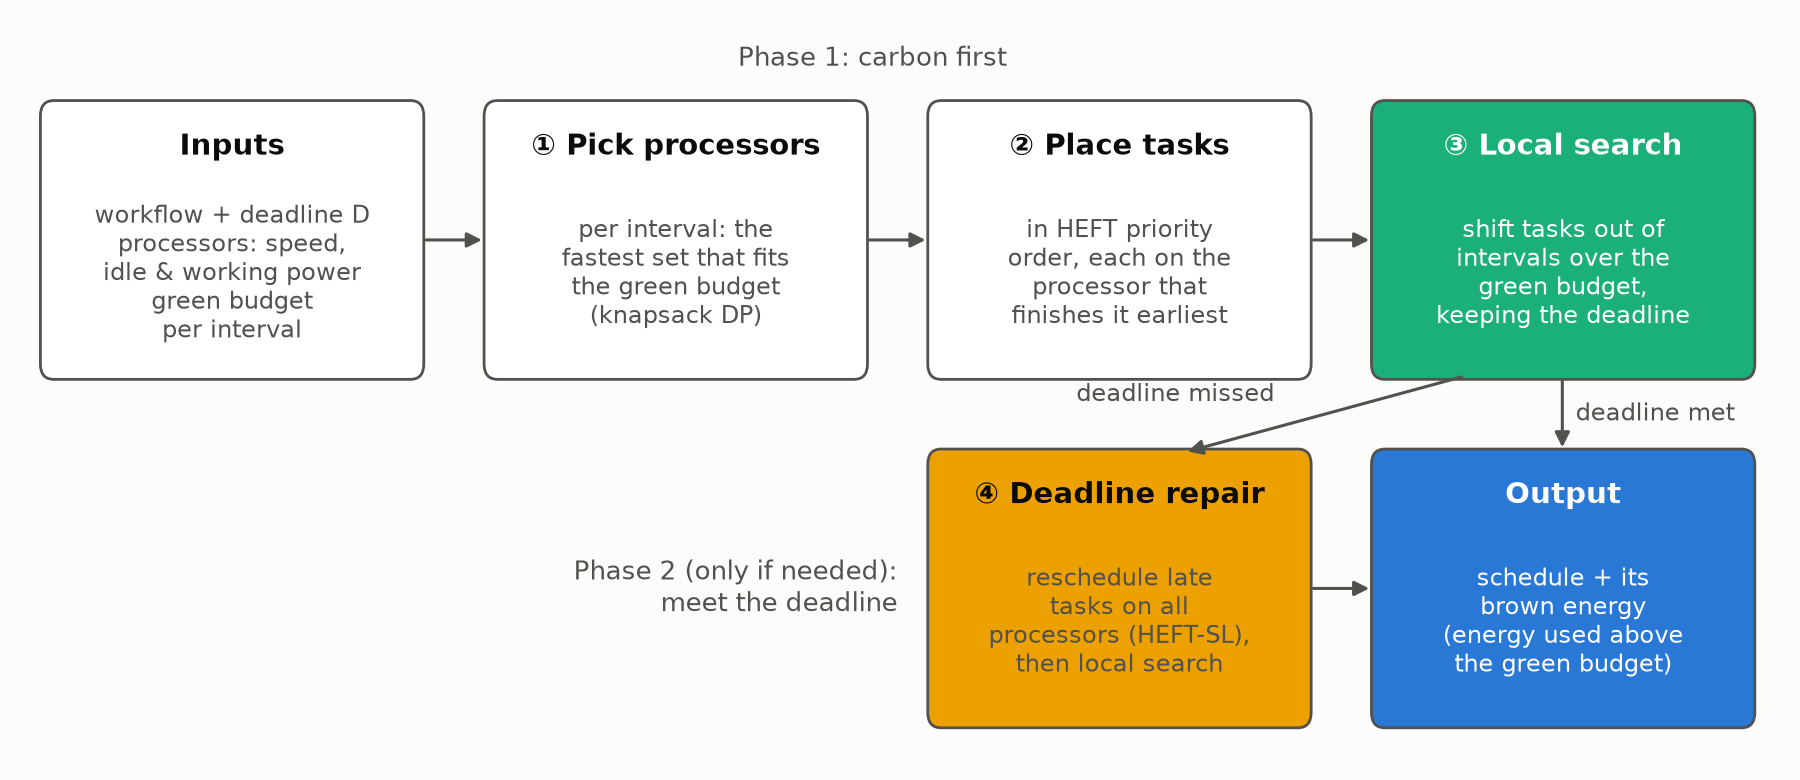
\includegraphics[width=\textwidth,keepaspectratio]{media/media/image1.png}
\caption[How CWM builds a schedule inside one data centre]{How CWM builds a schedule inside one data centre. Phase 1 favours carbon by limiting the processors to what the green budget allows; Phase 2 runs only if the deadline is missed.}\label{fig:2.1}
\end{figure}

In the authors\textquotesingle{} experiments, CWM cut carbon cost by
42--48 \% compared with CaWoSched and by 69 \% compared with
carbon-agnostic HEFT-SL, at the most relaxed deadlines tested (D = 2M)
{[}6{]}.

\textbf{How this project uses CWM.} We use CWM as a black box inside each DC. For every candidate (DC, transfer start) we give it that
DC\textquotesingle s processors, a power profile built from that
DC\textquotesingle s hourly CI (Section~\ref{sec:3.2}) that starts when the data
arrives, and the time left before the deadline, D\ensuremath{'}. CWM returns a
schedule and its energy in each interval, from which we compute the
carbon. Everything outside that box (choosing the DC, timing the
transfer, the network model, the theory and the evaluation) is this
project\textquotesingle s extension.

\section{Temporal shifting}\label{sec:2.3}

Wiesner \emph{et al.} {[}1{]} measured how much carbon delay-tolerant
jobs save by waiting for cleaner hours in Germany, Great Britain, France
and California. Their key observation is that the savings depend on how
much each grid varies over the day. CarbonScaler {[}2{]} grows and
shrinks elastic batch jobs with the carbon intensity instead of pausing
them, and Google {[}3{]} delays flexible work using day-ahead forecasts.
All three treat jobs as independent and none of them moves data.

\section{Spatial and spatiotemporal shifting}\label{sec:2.4}

CASPER {[}4{]} spreads web traffic across regions to cut carbon while
keeping latency low. A recent Kubernetes-based study {[}5{]} combines
spatial and temporal shifting for deadline-tolerant jobs and finds that
the difference between regions dominates the savings. Our results
explain why (Section~\ref{sec:6.2}).

\section{Carbon-aware data transfer}\label{sec:2.5}

LinTS {[}8{]} schedules transfers between cloud DCs over time with a
linear program and saves substantial carbon while meeting every transfer
deadline. Goldverg \emph{et al.} {[}9{]} measure the footprint of moving
data end to end and propose shifting transfers in time, space and route.
Sending a gigabyte was estimated to take 0.06 kWh in 2015, halving
roughly every two years {[}7{]}; we sweep this value rather than fix it
(Section~\ref{sec:5.3}). All of these optimise the transfer alone. The computation
that uses the data, and its deadline, are outside their model.

\begin{table}[htbp]
\centering
\caption[Decisions made by related approaches]{Decisions made by related approaches. (\ensuremath{\checkmark} = modelled, -- = not modelled).}\label{tab:2.1}
\begin{tabular}{@{}
  >{\raggedright\arraybackslash}p{(\columnwidth - 10\tabcolsep) * \real{0.3368}}
  >{\raggedright\arraybackslash}p{(\columnwidth - 10\tabcolsep) * \real{0.1263}}
  >{\raggedright\arraybackslash}p{(\columnwidth - 10\tabcolsep) * \real{0.1368}}
  >{\raggedright\arraybackslash}p{(\columnwidth - 10\tabcolsep) * \real{0.1263}}
  >{\raggedright\arraybackslash}p{(\columnwidth - 10\tabcolsep) * \real{0.1263}}
  >{\raggedright\arraybackslash}p{(\columnwidth - 10\tabcolsep) * \real{0.1476}}@{}}
\toprule\noalign{}
\begin{minipage}[b]{\linewidth}\raggedright
\textbf{Approach}
\end{minipage} & \begin{minipage}[b]{\linewidth}\raggedright
\textbf{Spatial (where)}
\end{minipage} & \begin{minipage}[b]{\linewidth}\raggedright
\textbf{Temporal compute}
\end{minipage} & \begin{minipage}[b]{\linewidth}\raggedright
\textbf{Transfer timing}
\end{minipage} & \begin{minipage}[b]{\linewidth}\raggedright
\textbf{DAG precedence}
\end{minipage} & \begin{minipage}[b]{\linewidth}\raggedright
\textbf{Shared deadline}
\end{minipage} \\
\midrule\noalign{}
HEFT {[}10{]} & -- & -- & -- & \ensuremath{\checkmark} & -- \\
CaWoSched {[}11{]}, CWM {[}6{]} & -- & \ensuremath{\checkmark} & -- & \ensuremath{\checkmark} & \ensuremath{\checkmark} (compute) \\
Let\textquotesingle s Wait Awhile {[}1{]}, CarbonScaler {[}2{]} & -- & \ensuremath{\checkmark}
& -- & -- & per job \\
CASPER {[}4{]} & \ensuremath{\checkmark} & -- & -- & -- & latency SLO \\
Kubernetes spatiotemporal {[}5{]} & \ensuremath{\checkmark} & \ensuremath{\checkmark} & -- & -- & per job \\
LinTS {[}8{]}, end-to-end data movement {[}9{]} & partly & -- & \ensuremath{\checkmark} & -- &
\ensuremath{\checkmark} (transfer) \\
\textbf{This work} & \ensuremath{\checkmark} & \ensuremath{\checkmark} (CWM) & \ensuremath{\checkmark} & \ensuremath{\checkmark} & \ensuremath{\checkmark} (end to end) \\
\bottomrule
\end{tabular}
\end{table}

\chapter{Problem Formulation}\label{ch:3}

\section{System model}\label{sec:3.1}

A workflow with \ensuremath{\Delta} GB of input starts at a source DC (Frankfurt in our
experiments). Several candidate DCs, including the source, could run it.
Each DC has its own processors and an hourly carbon-intensity (CI)
series in gCO\textsubscript{2}/kWh. Data moves to DC d at an effective rate
B\textsubscript{eff} (the link bandwidth times an efficiency \ensuremath{\eta}), so the
transfer takes \ensuremath{\tau} = \ensuremath{\Delta} / B\textsubscript{eff}. CWM measures time in whole
units of \ensuremath{\kappa} = 120 s (30 units per hour). The deadline is D = \ensuremath{\lceil}\ensuremath{\alpha}M\ensuremath{\rceil} units,
where M is the workflow\textquotesingle s HEFT makespan and \ensuremath{\alpha} \ensuremath{\geq}~1 says
how much slack the job has, as in {[}6{]}.

Three things are decided: the DC d, the time T\textsubscript{net} at
which the transfer starts, and the schedule inside d, which CWM chooses.
Computation can start only when all the data has arrived, and CWM gets
whatever is left of the deadline (Fig.~\ref{fig:3.1}):

\begin{equation}
T_{\mathrm{arr}} = \left\lceil \frac{T_{\mathrm{net}} + \Delta / B_{\mathrm{eff}}}{\kappa} \right\rceil, \qquad D' = D - T_{\mathrm{arr}}.\label{eq:3.1}
\end{equation}

\begin{figure}[htbp]
\centering
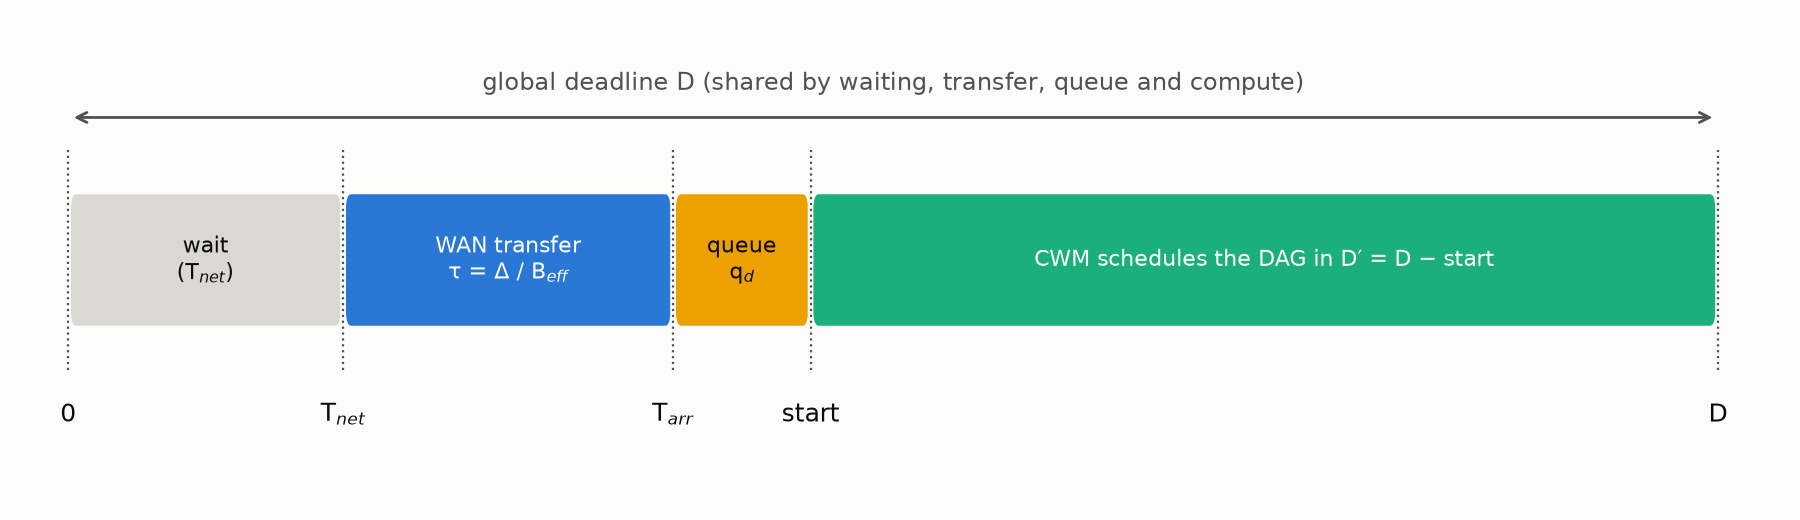
\includegraphics[width=\textwidth,keepaspectratio]{media/media/image2.png}
\caption[The deadline tension]{The deadline tension: waiting, transfer, queue (Section~\ref{sec:3.5}) and the CWM schedule all fit inside one global deadline D. Waiting longer or choosing a farther DC shrinks the window D\ensuremath{'} left for carbon-aware scheduling.}\label{fig:3.1}
\end{figure}

\section{Objective}\label{sec:3.2}

We minimise the total carbon of moving and computing, over every DC and
every allowed transfer start:

\begin{equation}
\min_{(d,\,T_{\mathrm{net}})} \; \mathrm{NetCarbon}_d(T_{\mathrm{net}}) + \mathrm{CompCarbon}_d(T_{\mathrm{arr}}).\label{eq:3.2}
\end{equation}

The latest allowed start still leaves enough time to run the workflow at
full speed. \textbf{Network carbon} charges \ensuremath{\varepsilon} kWh for every GB sent, at
the CI of the network during the transfer. We take that CI to be the
average of the source and destination grids, CI\textsuperscript{net}:

\begin{equation}
\mathrm{NetCarbon}_d(T) = \varepsilon\,\Delta \cdot \bigl(\text{average of } \mathrm{CI}^{\mathrm{net}} \text{ over the transfer from } T \text{ to } T+\tau\bigr).\label{eq:3.3}
\end{equation}

\textbf{Compute carbon} charges the energy the work adds on top of idle
power, at the DC\textquotesingle s grid CI in each interval j of the
schedule:

\begin{equation}
\mathrm{CompCarbon}_d = \sum_j k\bigl(E^{\mathrm{tot}}_j - P_{\mathrm{idle}}\,|I_j|\bigr) \cdot \mathrm{CI}_{d,j}.\label{eq:3.4}
\end{equation}

Here E\textsuperscript{tot}\textsubscript{j} is the energy
CWM\textquotesingle s schedule uses in interval j, and k(\ensuremath{\cdot}) converts
CWM\textquotesingle s energy units to kWh. CWM itself also needs a
\emph{green-power budget} for each interval: how much power it may use
while still counting as green. We derive it from the CI in the same way
for every DC, so cleaner hours give a larger budget:

\begin{equation}
\mathcal{G}_{d,j} = P_{\mathrm{idle}} + \max\bigl(0,\; 1 - \mathrm{CI}_{d,j}/800\bigr) \cdot f \cdot P_{\mathrm{dyn}}, \quad \text{with } f = 0.2.\label{eq:3.5}
\end{equation}

CWM optimises its own metric, the energy used \emph{above} this budget.
That metric has a blind spot, so we use it only as a secondary measure;
Section~\ref{sec:5.6} explains why.

\section{Three properties of the problem}\label{sec:3.3}

\begin{quote}
\textbf{Proposition 1 (waiting never makes computing cleaner).}
\emph{The best achievable compute carbon at a DC can only stay the same
or rise as the data arrives later.}
\end{quote}

Reason. The deadline is fixed. Any schedule that fits when the data
arrives later would also fit if the data arrived earlier, because the
earlier arrival gives the scheduler at least as much time. Waiting may
reduce network carbon, but it cannot improve the best possible compute
carbon. This is a property of the underlying optimisation problem; CWM
is a heuristic and does not follow it in every run. In our data, its
compute-carbon result decreases in 12--34\% of consecutive arrival
steps, so we include a control for solver variation (Section~\ref{sec:4.3}).\\
\strut \\
In practice: delaying a transfer can help the network, but it always
reduces the time available for computation.

\begin{quote}
\textbf{Proposition 2 (only a few start times need checking).}
\emph{With hourly CI data, the best transfer start for network carbon is
always either the earliest or latest allowed start, or a start where the
transfer begins or ends exactly on an hour boundary. Together with the
arrival-time steps, this finite set also contains the best start for the
total.}
\end{quote}

Reason. Carbon intensity is constant within each hour in our input data.
As the transfer start time moves within an hour, its network carbon
therefore changes linearly. The slope changes only when the transfer
starts or finishes in a different hour. The minimum must occur at one of
these change points or at the earliest or latest allowed start. Our
search checks these points, so it finds the minimum network carbon under
the hourly-data model.\\
\strut \\
In practice: we do not need to test every possible start time. We only
test the small set of times where the hourly carbon calculation can
change direction, together with the relevant arrival-time boundaries.

\begin{quote}
\textbf{Proposition 3 (long transfers gain less from waiting).} \emph{If
the network CI follows a daily cycle of amplitude A, the most that
waiting can save on network carbon is}
\end{quote}

\begin{equation}
2\,\varepsilon\,\Delta\,A\,\bigl|\mathrm{sinc}(\pi\tau / 24\,\mathrm{h})\bigr|, \quad \text{with } \mathrm{sinc}(x) = \sin(x)/x.\label{eq:3.6}
\end{equation}

Reason. A transfer averages the grid\textquotesingle s carbon intensity
over its entire duration. The longer the transfer, the more clean and
dirty hours it includes, so shifting its start time has less effect. For
a perfectly repeating daily cycle, this reduction is described by the
sinc factor in Eq.~(\ref{eq:3.6}); at a duration of 24 hours, shifting the
transfer provides no benefit. Real grids also vary with weather, so the
reduction is not as sharp as the ideal daily-cycle model predicts (Fig.
6.6).\\
\strut \\
In practice: waiting is most useful for short transfers on grids whose
carbon intensity changes substantially during the day.

\textbf{Complexity.} CWM\textquotesingle s own problem is the special
case with no data to move, and it is strongly NP-complete {[}6{]}, so
ours is strongly NP-hard. We therefore use CWM as a heuristic inside an
exact search over DCs and transfer starts.

\section{Different hardware}\label{sec:3.4}

In one study each DC has its own processor mix and its own power usage
effectiveness (PUE: total facility energy divided by IT energy). The
deadline is still set on the source DC\textquotesingle s hardware, and a
DC is usable only if its own HEFT makespan fits in the remaining window.
A higher PUE scales both carbon measures by exactly that factor, so the
scheduling problem inside the DC is unchanged and the three properties
still hold.

\section{Data-centre queues}\label{sec:3.5}

In another study a DC may have a queue: a job that arrives has to wait q
hours before it can start. This adds one new effect. If a queue empties
at an hour boundary, arriving just after it can start the computation
\emph{earlier} than arriving just before. So with queues, waiting can
sometimes reduce compute carbon too. These boundaries are already among
the start times checked by Proposition 2, so the search stays exact for
queue lengths in whole time units.

\section{Why place and time substitute}\label{sec:3.6}

Proposition 3 says that the benefit of waiting depends on how much a
data-centre\textquotesingle s electricity carbon intensity changes
during the day. In our data, the cleanest data centres have very stable
grids: hydro and nuclear power provide low-carbon electricity without
the strong daily pattern seen in solar-heavy grids. Once a workflow is
moved to one of these stable grids, there is little benefit in choosing
a particular computation time. The remaining opportunity comes mainly
from reducing network carbon, because the network carbon intensity still
reflects the source grid. This leads to a testable prediction: if the
stable, clean data centres are unavailable, joint scheduling should
provide a larger benefit. We test this in Section~\ref{sec:6.3}.

\section{A cheap estimate for ranking}\label{sec:3.7}

For RQ4 we want to rank all candidates without running CWM on each. We
estimate the total carbon of starting the transfer at time T at DC d as

\begin{multline}
\text{estimate} = \mathrm{NetCarbon}_d(T) + E \cdot \frac{\mathrm{PUE}_d}{\mathrm{PUE}_{\mathrm{ref}}} \\ \cdot \bigl(\text{mean CI of the } L \text{ cleanest hours left before the deadline}\bigr),\label{eq:3.7}
\end{multline}

where E is the job\textquotesingle s energy, taken from a single CWM
run, and L = \ensuremath{\lceil}M\ensuremath{\rceil} hours is how long the job needs at minimum. The
estimate is exact for the network and optimistic for the computation: it
pretends the job could run in the cleanest hours that remain, ignoring
task dependencies and the green budget. Like the real compute carbon, it
never improves as the start moves later.

\chapter{Methodology}\label{ch:4}

We followed four steps. First, we formulated the problem and proved the
properties in Chapter~\ref{ch:3}. These results tell us which transfer start
times need to be checked. Second, we built the search around the CWM
solver and tested the implementation, including the carbon calculations,
against values calculated by hand. Third, we ran the main experiments
using real 2024 electricity data. Finally, before each additional
experiment, we recorded what we expected to happen and reported whether
the results supported that expectation.

\section{System architecture}\label{sec:4.1}

Fig.~\ref{fig:4.1} shows the pipeline. Hourly CI data and the workflow and cluster
descriptions are combined into a \emph{topology}: the candidate DCs on
one shared clock, each with its CI, its green-power budget and, in some
studies, its hardware and queue. For each problem the optimiser lists
the candidate (DC, transfer start) pairs and evaluates every one
exactly: network carbon by formula, compute carbon by running CWM. Our
method and all the comparison strategies are then picked from the same
set of evaluations, so they are compared on identical numbers. The
Python package cwm\_multidc (about 3,700 lines) drives the CWM algorithm
through solve\_cwm, a small command-line front end we added to the CWM
C++ code.

\begin{figure}[p]
\centering
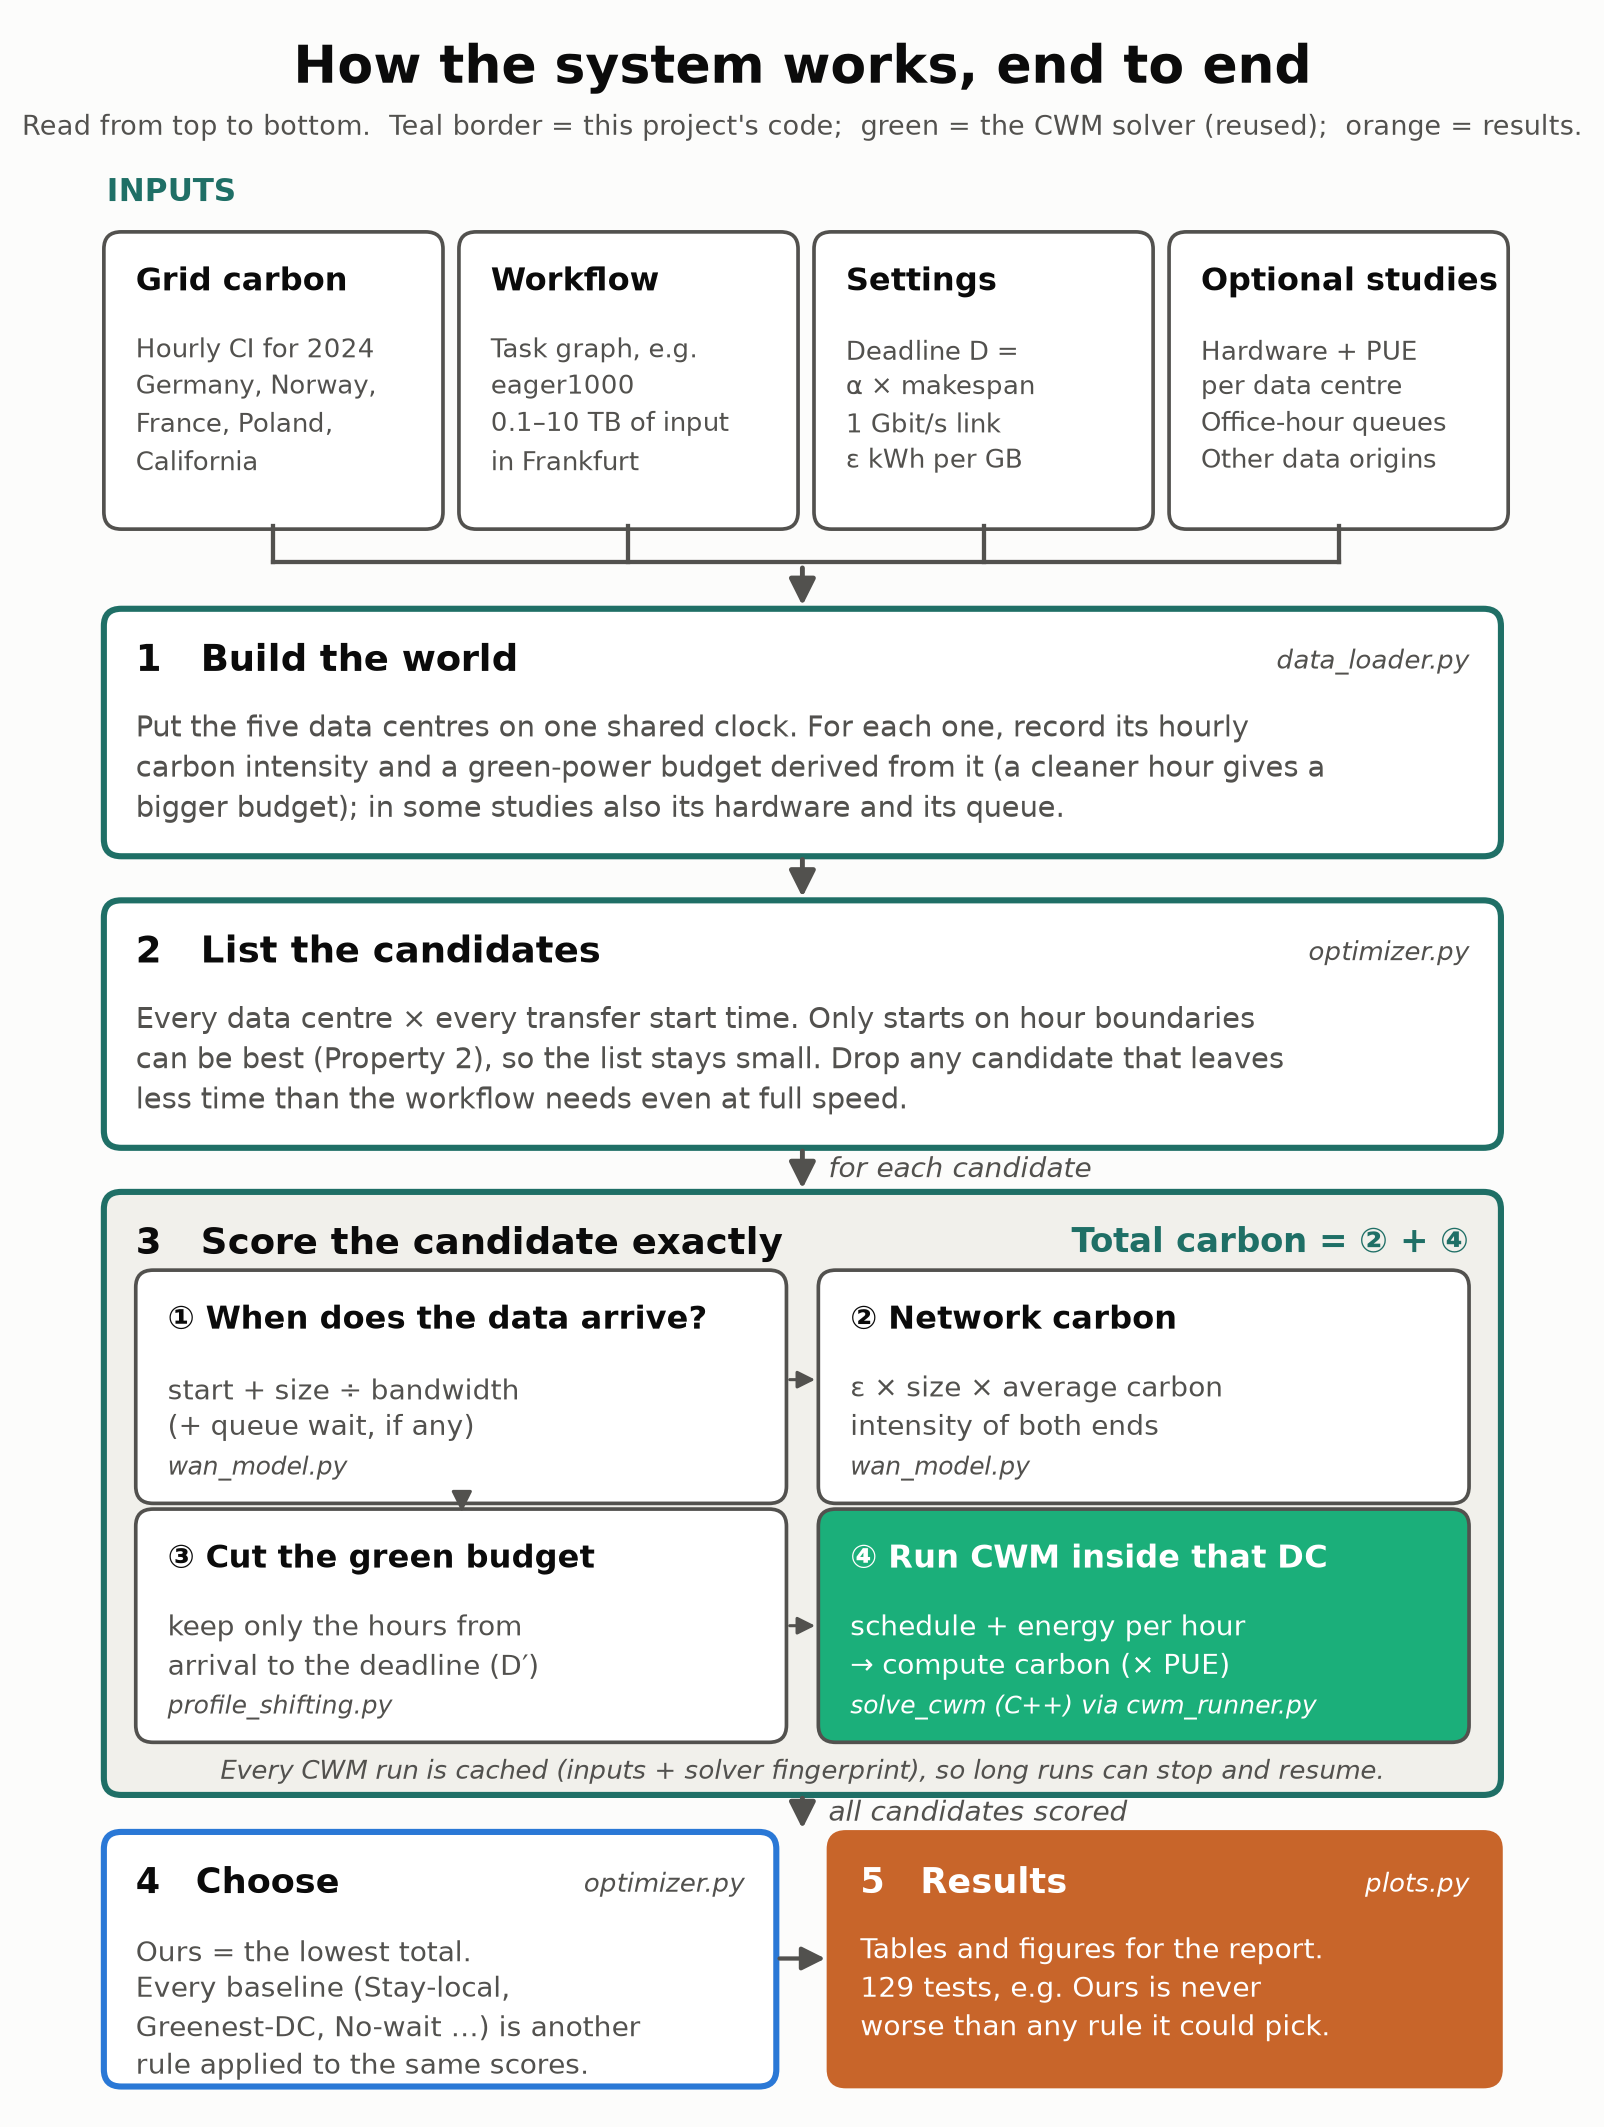
\includegraphics[width=\textwidth,height=0.86\textheight,keepaspectratio]{media/media/image11.png}
\caption[System architecture of the multi-DC extension]{System architecture of the multi-DC extension, read from top to bottom: the inputs, the five stages of the search, and the code file that performs each stage. Teal borders mark this project's code, green the reused CWM solver and orange the results.}\label{fig:4.1}
\end{figure}

\section{Joint search}\label{sec:4.2}

For each DC, the candidate transfer starts are the points from
Proposition 2 (the source DC only has ``start now'', since nothing
moves). Each candidate is evaluated in four steps:

\begin{enumerate}
\def\labelenumi{\arabic{enumi}.}
\item
  Work out when the data arrives (Eq.~(\ref{eq:3.1})) and, with queues, when
  computation can start (Section~\ref{sec:3.5}). Skip the candidate if the time
  left is shorter than the DC\textquotesingle s HEFT makespan.
\item
  Compute the network carbon of the transfer exactly (Eq.~(\ref{eq:3.3})).
\item
  Shift the DC\textquotesingle s power budget so that time zero is the
  moment computation can start, and cut it off at the deadline. The cut
  matters: CWM counts cost over the whole budget, idle power included,
  so without it the cost would depend on hours after the deadline.
\item
  Run solve\_cwm with the remaining deadline and compute the carbon of
  its schedule (Eq.~(\ref{eq:3.4})), scaled by the DC\textquotesingle s PUE.
\end{enumerate}

Algorithm~\ref{alg:joint} summarises the search.

\begin{algorithm}[htbp]
\caption{Joint search over data centres and transfer start times}\label{alg:joint}
\begin{algorithmic}[1]
\Require workflow $G$ with $\Delta$ GB of input at the source DC, deadline $D$, candidate DCs $\mathcal{D}$, hourly CI of every DC
\Ensure the lowest-carbon plan $(d, T_{\mathrm{net}})$ and its CWM schedule, i.e.\ Ours
\State $\mathit{best} \gets \text{none}$, \quad $C_{\mathit{best}} \gets \infty$
\ForAll{data centres $d \in \mathcal{D}$}
  \ForAll{transfer starts $T$ in the candidate set of Proposition~2}
    \State $T_{\mathrm{arr}} \gets \lceil (T + \Delta / B_{\mathrm{eff}}) / \kappa \rceil$, \quad $D' \gets D - T_{\mathrm{arr}}$ \Comment{Eq.~(\ref{eq:3.1})}
    \If{$D' < M_d$} \State \textbf{continue} \Comment{not enough time left to run}
    \EndIf
    \State $C_{\mathrm{net}} \gets \mathrm{NetCarbon}_d(T)$ \Comment{Eq.~(\ref{eq:3.3})}
    \State $\mathcal{G}' \gets$ green budget of $d$ from $T_{\mathrm{arr}}$ to the deadline
    \State $\sigma \gets \mathrm{CWM}(G, \mathcal{G}', D')$ \Comment{cached solver call}
    \State $C_{\mathrm{comp}} \gets \mathrm{CompCarbon}_d(\sigma)$ \Comment{Eq.~(\ref{eq:3.4})}
    \If{$C_{\mathrm{net}} + C_{\mathrm{comp}} < C_{\mathit{best}}$}
      \State $\mathit{best} \gets (d, T, \sigma)$, \quad $C_{\mathit{best}} \gets C_{\mathrm{net}} + C_{\mathrm{comp}}$
    \EndIf
  \EndFor
\EndFor
\State \Return $\mathit{best}$ \Comment{every baseline is read from the same scored candidates}
\end{algorithmic}
\end{algorithm}

We call the selected candidate Ours. The search checks all relevant
transfer start times and computes network carbon exactly under the
hourly-data model. However, because CWM is a heuristic, the overall
method is not guaranteed to find the globally optimal schedule.
Candidates run in parallel on eight workers. Each solver call is cached
on disk using its inputs and a SHA-256 fingerprint of the solver
program. This allows runs to be stopped and resumed, and prevents
results from a different solver build from being reused.

\section{What we compare against}\label{sec:4.3}

To know whether Ours is any good we need sensible alternatives. Table
4.1 lists them; the text uses the short names, and the codes are given
for reference. Each answers one question. \emph{Stay-local} shows what
not moving costs. \emph{Greenest-DC + HEFT} shows what a carbon-unaware
scheduler costs. \emph{Greenest-DC}, the obvious strategy of sending the
data now to the cleanest site, is the main yardstick.
\emph{Network-only} and \emph{Compute-only} optimise just one half of
the problem. \emph{Efficiency-aware} and \emph{Queue-aware} are fair
rivals for the hardware and queue studies.

Two ablations take Ours apart. \emph{No-wait} chooses the DC but never
waits; \emph{Fixed-DC} waits but always uses the greenest DC. Finally,
the \emph{Equal-budget control} guards against solver luck. Ours calls
CWM many times per problem and keeps the best result, while Greenest-DC
calls it once. Since CWM is a noisy heuristic, some of
Ours\textquotesingle{} advantage could come from simply trying more
often. The control runs Greenest-DC as many times as Ours does, with
different random seeds, and keeps its best; a gain that survives this is
not luck. Except for Greenest-DC + HEFT and the control, every strategy
is one of Ours\textquotesingle{} own candidates, so Ours can never do
worse than them, and an automated test checks this on every saved
result.

\begin{table}[htbp]
\centering
\caption[Comparison strategies]{Comparison strategies. ``Send now'' means the transfer starts immediately.}\label{tab:4.1}
\begin{tabular}{@{}
  >{\raggedright\arraybackslash}p{(\columnwidth - 4\tabcolsep) * \real{0.1010}}
  >{\raggedright\arraybackslash}p{(\columnwidth - 4\tabcolsep) * \real{0.2359}}
  >{\raggedright\arraybackslash}p{(\columnwidth - 4\tabcolsep) * \real{0.6631}}@{}}
\toprule\noalign{}
\begin{minipage}[b]{\linewidth}\raggedright
\textbf{Code}
\end{minipage} & \begin{minipage}[b]{\linewidth}\raggedright
\textbf{Name}
\end{minipage} & \begin{minipage}[b]{\linewidth}\raggedright
\textbf{What it does}
\end{minipage} \\
\midrule\noalign{}
B1 & Stay-local & Run at the source DC; nothing is moved \\
B2 & Greenest-DC + HEFT & Send now to the DC with the lowest average CI;
plain, carbon-unaware HEFT schedule \\
B3 & Greenest-DC & As above but with the CWM schedule (the main
yardstick) \\
B4 & Network-only & Greenest DC, transfer start with the lowest network
carbon \\
B5 & Compute-only & Send now to every DC, pick the one with the lowest
compute carbon \\
B6 & Efficiency-aware & Send now to the DC with the lowest PUE \ensuremath{\times} average
CI \\
B7 & Queue-aware & Send now to the greenest DC that can still meet the
deadline after its queue \\
A1 & No-wait & Ours without waiting: best DC, transfer starts now \\
A2 & Fixed-DC & Ours without choosing the DC: greenest DC, best transfer
start \\
C1 & Equal-budget control & Greenest-DC run with as many solver calls as
Ours, best kept \\
R1 / R3 & Cheap rule & Rank all candidates with the estimate of Section
3.7 and solve only the best 1 / 3 \\
\bottomrule
\end{tabular}
\end{table}

\section{The cheap rule}\label{sec:4.4}

The cheap rule turns the estimate of Section~\ref{sec:3.7} into a strategy. It
runs CWM once to measure the job\textquotesingle s energy, ranks every
candidate with the estimate, and then runs CWM only on the best one (at
most 2 solver calls in total) or the best three (at most 4).

We changed the rule once. The first version took the
job\textquotesingle s length from that single CWM run. But CWM stretches
a schedule to fill whatever window it is given, so every wait looked
expensive and the rule waited too little. Using the
workflow\textquotesingle s minimum duration instead, as the theory
suggests, fixed this. After that change we froze the rule, and the
hardware, queue, no-flat-grid and data-origin studies serve as tests it
had never seen.

\section{Testing and reproducibility}\label{sec:4.6}

The package has 129 automated tests. They check the budget shifting, the
network formula and the solver output parsing; the carbon arithmetic
against hand-computed values; the list of transfer starts against a
brute-force search; full runs of the real solver; the hardware, queue
and rule extensions; and, on every saved study, that Ours is never worse
than a strategy it could have chosen. Each results folder records where
the CI data came from, the solver\textquotesingle s fingerprint and the
git commit. reproduce\_multidc.sh rebuilds the solver and regenerates
every result, and run\_chunks.sh splits the run into sessions that can
be stopped and resumed. The CI data can be rebuilt from the public
sources with python -m cwm\_multidc.scripts.fetch\_public\_ci.

\textbf{Source code.} Everything (the CWM solver, the cwm\_multidc
package, the 2024 CI data, all result files and the sources of this
report) is on GitHub at
\url{https://github.com/tuhina2005/carbon-aware-multidc-scheduling}.
The repository\textquotesingle s README lists the commands that rebuild
every table and figure, and python -m unittest discover -s
cwm\_multidc/tests -t . runs the tests.

\chapter{Datasets and Experimental Setup}\label{ch:5}

\section{Carbon-intensity data}\label{sec:5.1}

All experiments use real hourly data for 2024 from five regions.
Germany, France, Poland and Norway come from Energy-Charts (ENTSO-E
data) {[}12{]}, and California from the CAISO grid operator {[}13{]}.
For each hour we compute the CI as the average of standard emission
factors per fuel {[}14{]} (coal 820, gas 490, oil 650, biomass 230,
solar 45, geothermal 38, hydro 24, nuclear 12, wind 11 gCO\textsubscript{2}/kWh),
weighted by how much each fuel generated. Sixteen California hours were
missing (gaps of at most 12 hours) and are filled by interpolation; no
other region has gaps. We planned to include India, but no free hourly
data exists, so there are five DCs: Frankfurt (where the data starts),
Oslo, Paris, Warsaw and California.

Table~\ref{tab:5.1} summarises the data. Look at the last two columns, which show
how much each grid swings within a day: the two cleanest grids are also
almost flat. This turns out to drive the results in Chapter~\ref{ch:6}.

\begin{table}[htbp]
\centering
\caption[Carbon-intensity statistics of the five regions (2024)]{Carbon-intensity statistics of the five regions (2024). The five regions in 2024: mean carbon intensity, median daily swing (max \ensuremath{-} min within a day) and median amplitude A of the 24-hour harmonic (gCO\textsubscript{2}/kWh).}\label{tab:5.1}
\begin{tabular}{@{}
  >{\raggedright\arraybackslash}p{(\columnwidth - 8\tabcolsep) * \real{0.2890}}
  >{\raggedright\arraybackslash}p{(\columnwidth - 8\tabcolsep) * \real{0.2168}}
  >{\raggedright\arraybackslash}p{(\columnwidth - 8\tabcolsep) * \real{0.1445}}
  >{\raggedright\arraybackslash}p{(\columnwidth - 8\tabcolsep) * \real{0.1565}}
  >{\raggedright\arraybackslash}p{(\columnwidth - 8\tabcolsep) * \real{0.1931}}@{}}
\toprule\noalign{}
\begin{minipage}[b]{\linewidth}\raggedright
\textbf{DC (region)}
\end{minipage} & \begin{minipage}[b]{\linewidth}\raggedright
\textbf{Main sources}
\end{minipage} & \begin{minipage}[b]{\linewidth}\raggedright
\textbf{Mean CI}
\end{minipage} & \begin{minipage}[b]{\linewidth}\raggedright
\textbf{Daily swing}
\end{minipage} & \begin{minipage}[b]{\linewidth}\raggedright
\textbf{24 h amplitude A}
\end{minipage} \\
\midrule\noalign{}
Oslo (NO) & hydro & 29.9 & 3 & 0.7 \\
Paris (FR) & nuclear & 36.1 & 10 & 3.2 \\
California (US-CAL) & gas, solar & 196.4 & 158 & 74.7 \\
Frankfurt (DE), source & wind, coal, solar & 319.7 & 191 & 71.6 \\
Warsaw (PL) & coal & 560.3 & 232 & 88.0 \\
\bottomrule
\end{tabular}
\end{table}

\section{Workflows and clusters}\label{sec:5.2}

We use real bioinformatics workflows from WfCommons {[}15{]} that come
with CWM: atacseq200 (200 tasks, 5.6 hours at full speed) and eager1000
(1,000 tasks, 11.2 hours) in every study, plus chipseq1000 and
methylseq1000 in the headline study. Every DC runs CWM\textquotesingle s
``small'' cluster (72 processors of six types) unless stated otherwise.
The hardware study uses three kinds of DC: \emph{efficient} (the three
most efficient processor types, PUE 1.10, the level Google reports
{[}16{]}); \emph{standard} (all six types, PUE 1.55, close to the 2024
industry average of 1.56 {[}17{]}); and an illustrative \emph{legacy} DC
(slower, less efficient types, PUE 2.00).

\section{Parameters}\label{sec:5.3}

Table~\ref{tab:5.2} lists the settings. Values in brackets were varied to test how
sensitive the results are.

\begin{table}[htbp]
\centering
\caption[Model parameters]{Model parameters. Values in brackets are swept.}\label{tab:5.2}
\begin{tabular}{@{}
  >{\raggedright\arraybackslash}p{(\columnwidth - 4\tabcolsep) * \real{0.2500}}
  >{\raggedright\arraybackslash}p{(\columnwidth - 4\tabcolsep) * \real{0.2272}}
  >{\raggedright\arraybackslash}p{(\columnwidth - 4\tabcolsep) * \real{0.5228}}@{}}
\toprule\noalign{}
\begin{minipage}[b]{\linewidth}\raggedright
\textbf{Parameter}
\end{minipage} & \begin{minipage}[b]{\linewidth}\raggedright
\textbf{Default}
\end{minipage} & \begin{minipage}[b]{\linewidth}\raggedright
\textbf{Notes}
\end{minipage} \\
\midrule\noalign{}
Time unit \ensuremath{\kappa} & 120 s (30 units = 1 h) & {[}60, 120, 240 s{]}; calibrates
one CWM interval to one CI hour \\
WAN bandwidth B, efficiency \ensuremath{\eta} & 1 Gbit/s, 0.95 & {[}0.5--10 Gbit/s{]} \\
Network energy \ensuremath{\varepsilon} & 0.02 kWh/GB & {[}0.001, 0.005, 0.02, 0.06{]}; \ensuremath{\approx}~0.003
is the 2024 extrapolation of {[}7{]} \\
Green fraction f & 0.2 & CWM small-cluster setting \\
Deadline factor \ensuremath{\alpha} & 1.5, 2.0, 2.5 & {[}1.2--2.5{]} in the single-day
grid \\
Input volume \ensuremath{\Delta} & 100 GB, 1 TB & {[}100 GB--10 TB{]} in the single-day
grid \\
CWM seeds & 42 & 42/43/44 in the headline and noise-control runs \\
\bottomrule
\end{tabular}
\end{table}

The energy cost of the network, \ensuremath{\varepsilon}, is the assumption that matters most.
Our default of 0.02 kWh/GB matches roughly 2018 on the trend of {[}7{]};
today\textquotesingle s value is closer to 0.003. So we recompute every
result for the whole range, and report the key result at \ensuremath{\varepsilon} = 0.001 too.

\section{Studies}\label{sec:5.4}

Table~\ref{tab:5.3} lists the studies. The first four measure the gain; the rest
test the explanation and stress the method. Before running each of
those, we wrote down what we expected (last column).

\begin{table}[htbp]
\centering
\caption[Experimental studies]{Experimental studies (all on real 2024 CI). Dates are the third Wednesdays of the months named.}\label{tab:5.3}
\begin{tabular}{@{}
  >{\raggedright\arraybackslash}p{(\columnwidth - 6\tabcolsep) * \real{0.1777}}
  >{\raggedright\arraybackslash}p{(\columnwidth - 6\tabcolsep) * \real{0.1110}}
  >{\raggedright\arraybackslash}p{(\columnwidth - 6\tabcolsep) * \real{0.3999}}
  >{\raggedright\arraybackslash}p{(\columnwidth - 6\tabcolsep) * \real{0.3114}}@{}}
\toprule\noalign{}
\begin{minipage}[b]{\linewidth}\raggedright
\textbf{Study}
\end{minipage} & \begin{minipage}[b]{\linewidth}\raggedright
\textbf{Problems}
\end{minipage} & \begin{minipage}[b]{\linewidth}\raggedright
\textbf{Design}
\end{minipage} & \begin{minipage}[b]{\linewidth}\raggedright
\textbf{Question / expectation}
\end{minipage} \\
\midrule\noalign{}
Single-day grid & 70 & 2 workflows \ensuremath{\times} 5 data sizes \ensuremath{\times} 7 deadlines; 17 Apr,
06 UTC & Where does each choice win? \\
Headline & 16 & 4 workflows \ensuremath{\times} 2 start hours \ensuremath{\times} 2 deadlines; 1 TB; 3 seeds
& Larger workflows; solver noise \\
Sensitivity & 16 & Time unit, bandwidth, forecast error & How sensitive
are the results? \\
Year-round & 192 & Jan/Apr/Jul/Oct \ensuremath{\times} 0/6/12/18 UTC \ensuremath{\times} 2 workflows \ensuremath{\times} 2
sizes \ensuremath{\times} 3 deadlines & Does the picture hold all year? \\
Noise control & 21 & Year-round winners (\ensuremath{\geq}~5~\%), 3 seeds + equal-budget
control & Are the wins solver luck? \\
No flat clean grid & 192 paired & Year-round, with only Frankfurt,
Warsaw and California & Expected: larger gain \\
Hardware & 96 & 4 hardware scenarios \ensuremath{\times} Jan/Jul \ensuremath{\times} 06 UTC & Expected:
greenest-DC loses \ensuremath{\geq}~10~\% \\
Queues & 192 & Daily queues at 3 busyness levels \ensuremath{\times} Jan/Jul \ensuremath{\times} 4 hours &
Expected: gain grows with busyness \\
Data origin & 192 & Data starting in Frankfurt / Warsaw / California \ensuremath{\times}
64 & Expected: waiting follows the source grid\textquotesingle s
swing \\
\bottomrule
\end{tabular}
\end{table}

\section{How results are reported}\label{sec:5.5}

For any strategy X we report the gain of Ours,

\begin{equation}
\mathrm{gain}(X) = 1 - C_{\mathrm{Ours}} / C_X,\label{eq:5.1}
\end{equation}

where C is total carbon (network plus compute). A gain of 5~\% means
Ours emits 5~\% less CO\textsubscript{2} than X. We report the mean, median and maximum
over problems, and the share of problems where the gain is at least
5~\%. When two settings are compared, each problem is paired with its
twin. Unless stated otherwise, \ensuremath{\varepsilon} = 0.02 kWh/GB.

\section{A note on CWM\textquotesingle s own metric}\label{sec:5.6}

All results use the carbon measure of Section~\ref{sec:3.2}, which charges the
energy the work actually uses at the grid\textquotesingle s CI.
CWM\textquotesingle s own objective is different: it counts only the
energy used \emph{above} the green-power budget (``brown'' energy).
Because that budget is itself derived from the CI, a job that fits under
it scores zero, however dirty the grid. On real data this makes the
brown measure prefer Frankfurt (\ensuremath{\approx}~320 gCO\textsubscript{2}/kWh) to Paris (\ensuremath{\approx}~36) for
small jobs, which is clearly wrong as a carbon measure. We therefore
report it only here.

Measured this way, Ours appears to beat Greenest-DC by 37.6~\% over the
year, but almost all of that comes from small atacseq200 jobs that stay
in Frankfurt with zero brown energy. The cheap rule, which ignores the
budget, captures only 27~\% of the gain under this measure. None of the
conclusions in Chapter~\ref{ch:6} depend on it.

\chapter{Results}\label{ch:6}

We organise the results as four questions. Does joint scheduling help
(6.1)? Why is the gain small (6.2)? When does it pay off (6.3)? Does it
hold under harder conditions, and can a cheap rule get most of it (6.4,
6.5)? We then list what happened to each expectation (6.6), discuss the
results (6.7) and compare them with earlier work (6.8).

\section{Does joint scheduling help?}\label{sec:6.1}

\textbf{Yes, but most of the benefit comes from choosing the place;
choosing the time adds a small 1.8~\% on average.}

\subsection{A single day}

Fig.~\ref{fig:6.1} shows what Ours chooses on 17 April 2024 for every data size
and deadline. Very large inputs (10 TB, and 3 TB with tight deadlines)
cannot be moved in time, so everything runs in Frankfurt. Everywhere
else the job moves to Paris. When the input is small or medium and the
deadline has slack, Ours also \emph{waits}, so that the transfer runs
during Frankfurt\textquotesingle s sunny midday, and gains up to 23~\%
over Greenest-DC on atacseq200 and up to 11~\% on eager1000. Over the 70
problems Ours beats Stay-local by 53.7~\% on average and Greenest-DC by
4.2~\% (27~\% of problems at least 5~\%, best 22.7~\%).

Fig.~\ref{fig:6.2} shows the deadline tension in one problem. Network-only finds
the cheapest network slot but squeezes the computation, while Ours finds
the best balance between the two.

\begin{figure}[htbp]
\centering
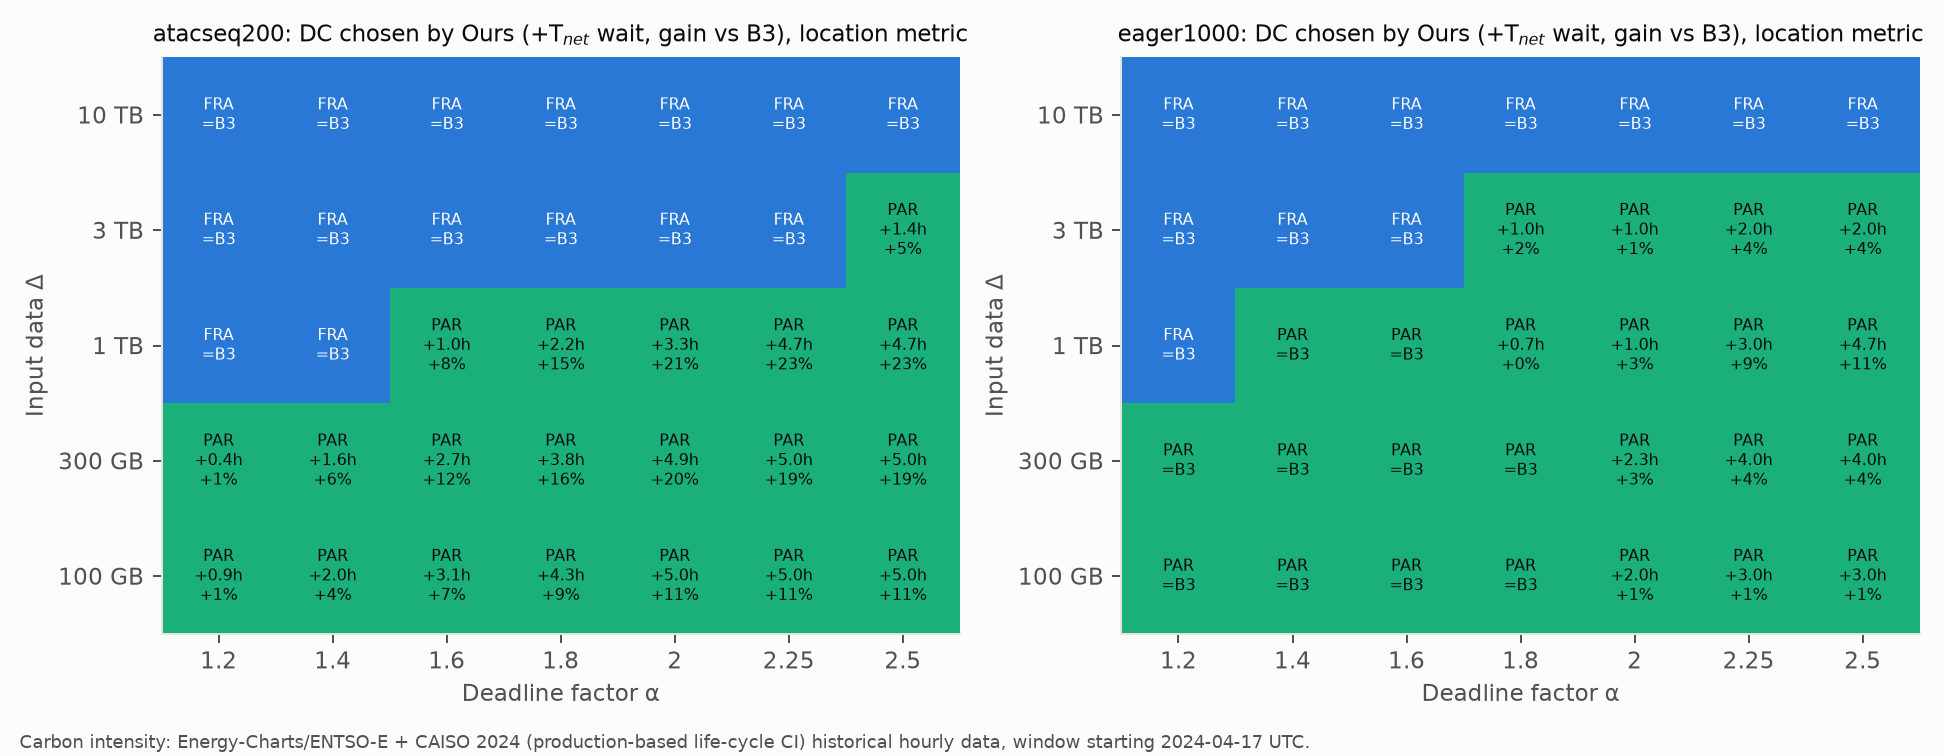
\includegraphics[width=\textwidth,keepaspectratio]{media/media/image4.png}
\caption[What Ours chooses on a single day (17 April 2024)]{What Ours chooses on a single day (17 April 2024). Phase diagram on 17 April 2024: the DC Ours chooses, how long it waits, and its gain over Greenest-DC (B3 in the figure), for each data volume and deadline factor.}\label{fig:6.1}
\end{figure}

\begin{figure}[htbp]
\centering
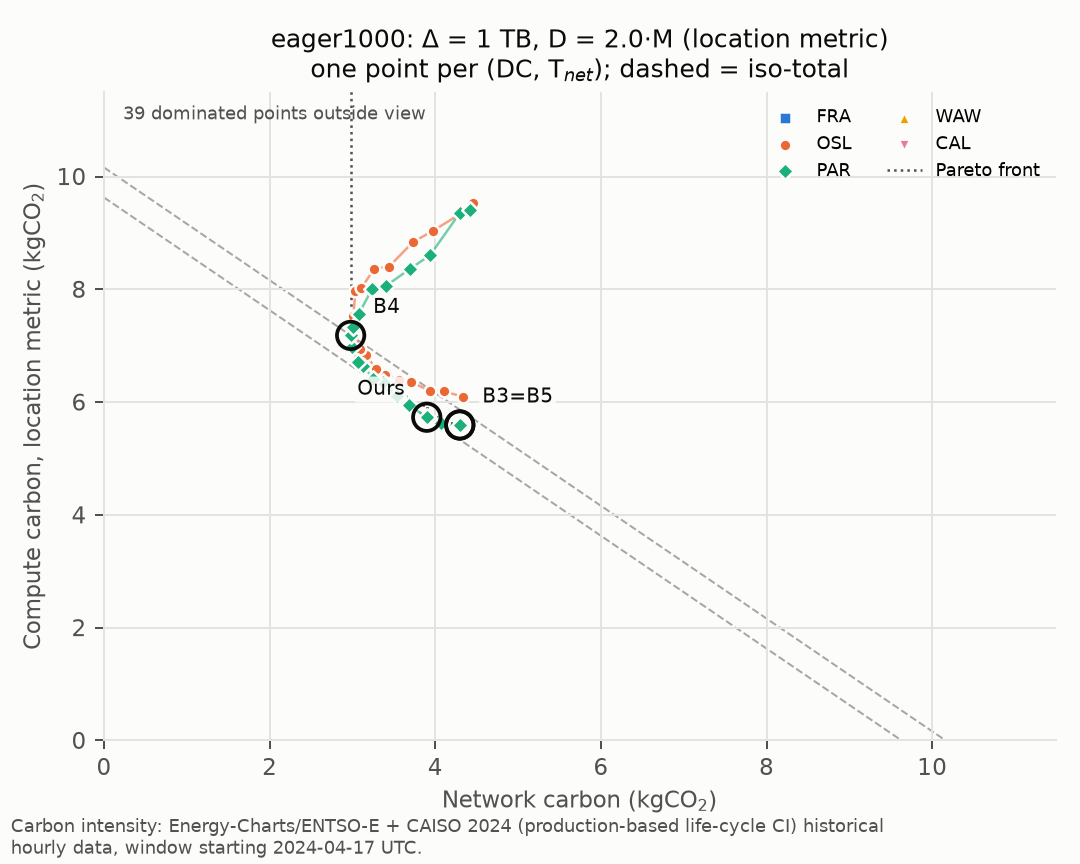
\includegraphics[width=5.4in,keepaspectratio]{media/media/image5.png}
\caption[Network versus compute carbon of every candidate]{Network vs compute carbon of every candidate (DC, transfer start) for eager1000, 1 TB, \ensuremath{\alpha} = 2. Dashed lines have equal total carbon; circles mark Ours, Greenest-DC (B3), Network-only (B4) and Compute-only (B5).}\label{fig:6.2}
\end{figure}

\subsection{Across the year}

Table~\ref{tab:6.1} and Fig.~\ref{fig:6.3} repeat this on four days spread over the year, at
four submission hours. Ours emits 83.9~\% less than Stay-local and
16.1~\% less than Greenest-DC + HEFT. Against Greenest-DC, though, the
joint search saves only \textbf{1.8~\%} on average (median 0; at least
5~\% in 11~\% of problems).

Ours picks the same DC as Greenest-DC in 93~\% of problems. It waits in
42~\% of them, and when it does, waiting saves 3.8~\% compared with
sending at once. The gains cluster at 06:00 UTC submissions in spring
and summer, when a short wait lets the transfer run over
Germany\textquotesingle s solar midday. Fixed-DC is within 0.2~\% of
Ours, so almost all of Ours\textquotesingle{} advantage over Greenest-DC
comes from \emph{waiting}, not from a better choice of DC.

\begin{table}[htbp]
\centering
\caption[Year-round results (192 problems)]{Year-round results: gain of Ours over each strategy (192 problems, \ensuremath{\varepsilon} = 0.02).}\label{tab:6.1}
\begin{tabular}{@{}
  >{\raggedright\arraybackslash}p{(\columnwidth - 8\tabcolsep) * \real{0.3750}}
  >{\raggedright\arraybackslash}p{(\columnwidth - 8\tabcolsep) * \real{0.1499}}
  >{\raggedright\arraybackslash}p{(\columnwidth - 8\tabcolsep) * \real{0.1499}}
  >{\raggedright\arraybackslash}p{(\columnwidth - 8\tabcolsep) * \real{0.1499}}
  >{\raggedright\arraybackslash}p{(\columnwidth - 8\tabcolsep) * \real{0.1752}}@{}}
\toprule\noalign{}
\begin{minipage}[b]{\linewidth}\raggedright
\textbf{Strategy}
\end{minipage} & \begin{minipage}[b]{\linewidth}\raggedright
\textbf{Mean~\%}
\end{minipage} & \begin{minipage}[b]{\linewidth}\raggedright
\textbf{Median~\%}
\end{minipage} & \begin{minipage}[b]{\linewidth}\raggedright
\textbf{Max~\%}
\end{minipage} & \begin{minipage}[b]{\linewidth}\raggedright
\textbf{Share \ensuremath{\geq}~5~\%}
\end{minipage} \\
\midrule\noalign{}
Stay-local (B1) & 83.9 & 87.9 & 95.6 & 100~\% \\
Greenest-DC + HEFT (B2) & 16.1 & 12.4 & 39.5 & 64~\% \\
Greenest-DC (B3) & 1.8 & 0.0 & 22.7 & 11~\% \\
Network-only (B4) & 4.9 & 0.1 & 41.4 & 26~\% \\
Compute-only (B5) & 1.6 & 0.0 & 22.7 & 9~\% \\
No-wait (A1) & 1.6 & 0.0 & 22.7 & 9~\% \\
Fixed-DC (A2) & 0.2 & 0.0 & 10.4 & 2~\% \\
Cheap rule, top 3 (R3) & 0.4 & 0.0 & 5.5 & 1~\% \\
\bottomrule
\end{tabular}
\end{table}

\begin{figure}[htbp]
\centering
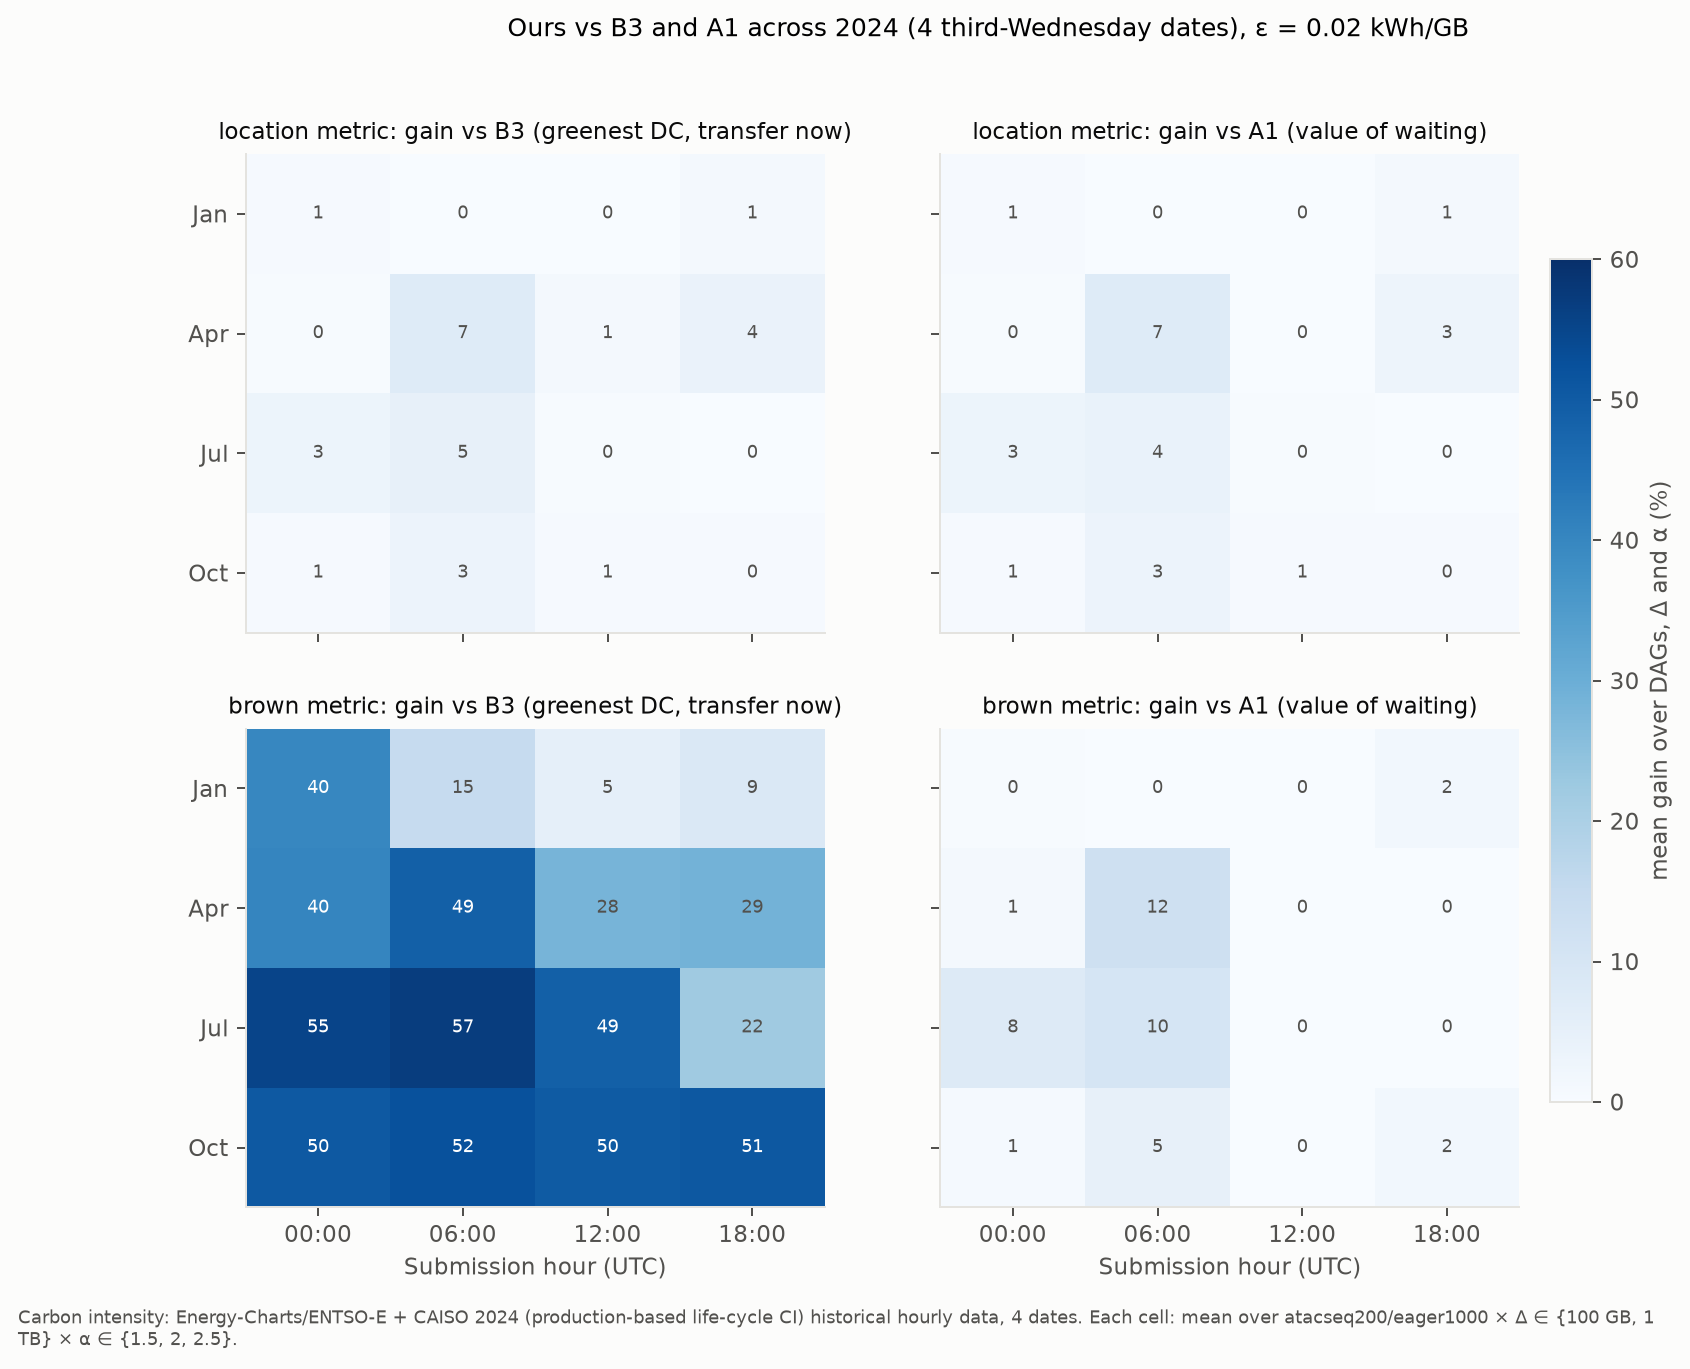
\includegraphics[width=\textwidth,keepaspectratio]{media/media/image6.png}
\caption[Year-round gain by month and submission hour]{Year-round gain by month and submission hour. Mean gain of Ours over Greenest-DC (B3, left) and over No-wait (A1, right), i.e. the value of waiting, by month and submission hour. The top row uses our carbon measure; the bottom row uses CWM\textquotesingle s own brown measure (Section~\ref{sec:5.6}).}\label{fig:6.3}
\end{figure}

\subsection{Are the wins real?}

Yes. Table~\ref{tab:6.2} re-solves the 21 problems where Ours won by at least
5~\%, with three seeds and the Equal-budget control. Ours keeps an
11.2~\% mean gain over the control, at least 5~\% in every one of them
and never a loss, so these are not lucky solver runs. The wins come from
the network: where Ours waits at the same DC, network carbon falls by
12.4 kg in total while compute carbon rises by only 0.6 kg.

\begin{table}[htbp]
\centering
\caption[Noise control on the year-round winners]{Noise control on the 21 year-round problems where Ours beat Greenest-DC by \ensuremath{\geq}~5~\%.}\label{tab:6.2}
\begin{tabular}{@{}
  >{\raggedright\arraybackslash}p{(\columnwidth - 8\tabcolsep) * \real{0.3908}}
  >{\raggedright\arraybackslash}p{(\columnwidth - 8\tabcolsep) * \real{0.1609}}
  >{\raggedright\arraybackslash}p{(\columnwidth - 8\tabcolsep) * \real{0.1609}}
  >{\raggedright\arraybackslash}p{(\columnwidth - 8\tabcolsep) * \real{0.1493}}
  >{\raggedright\arraybackslash}p{(\columnwidth - 8\tabcolsep) * \real{0.1382}}@{}}
\toprule\noalign{}
\begin{minipage}[b]{\linewidth}\raggedright
\textbf{Comparison}
\end{minipage} & \begin{minipage}[b]{\linewidth}\raggedright
\textbf{Mean gain~\%}
\end{minipage} & \begin{minipage}[b]{\linewidth}\raggedright
\textbf{Median gain~\%}
\end{minipage} & \begin{minipage}[b]{\linewidth}\raggedright
\textbf{Share \ensuremath{\geq}~5~\%}
\end{minipage} & \begin{minipage}[b]{\linewidth}\raggedright
\textbf{Share \ensuremath{\leq}~0}
\end{minipage} \\
\midrule\noalign{}
Ours vs Greenest-DC, one seed & 11.2 & -- & 100~\% & 0~\% \\
Ours vs Greenest-DC, three seeds & 11.2 & -- & 100~\% & 0~\% \\
Ours vs Equal-budget control & 11.2 & 10.9 & 100~\% & 0~\% \\
\bottomrule
\end{tabular}
\end{table}

\subsection{Sensitivity}

Fig.~\ref{fig:6.4} changes one setting at a time (eager1000, 1 TB, \ensuremath{\alpha} = 2). A
faster network makes waiting cheaper: the gain over Greenest-DC rises
from 0 at 0.5 Gbit/s to 10.9~\% at 10 Gbit/s. The time unit matters too
(6.6~\% at 240 s, 2.6~\% at 120 s, 1.7~\% at 60 s), because compute
energy scales with it and network energy does not. Cheaper networks
shrink the gain but do not remove it: over the year it is 1.1~\% at \ensuremath{\varepsilon} =
0.001, 1.3~\% at 0.005, 1.8~\% at 0.02 and 2.9~\% at 0.06. The one real
weakness is forecast error. With slightly noisy CI forecasts Ours still
gains (+1.9~\% at \ensuremath{\sigma} = 0.1), but with very noisy ones (\ensuremath{\sigma} = 0.5) it does
\emph{worse} than Greenest-DC, by 8.8~\% on average and 16~\% at worst.

\begin{figure}[htbp]
\centering
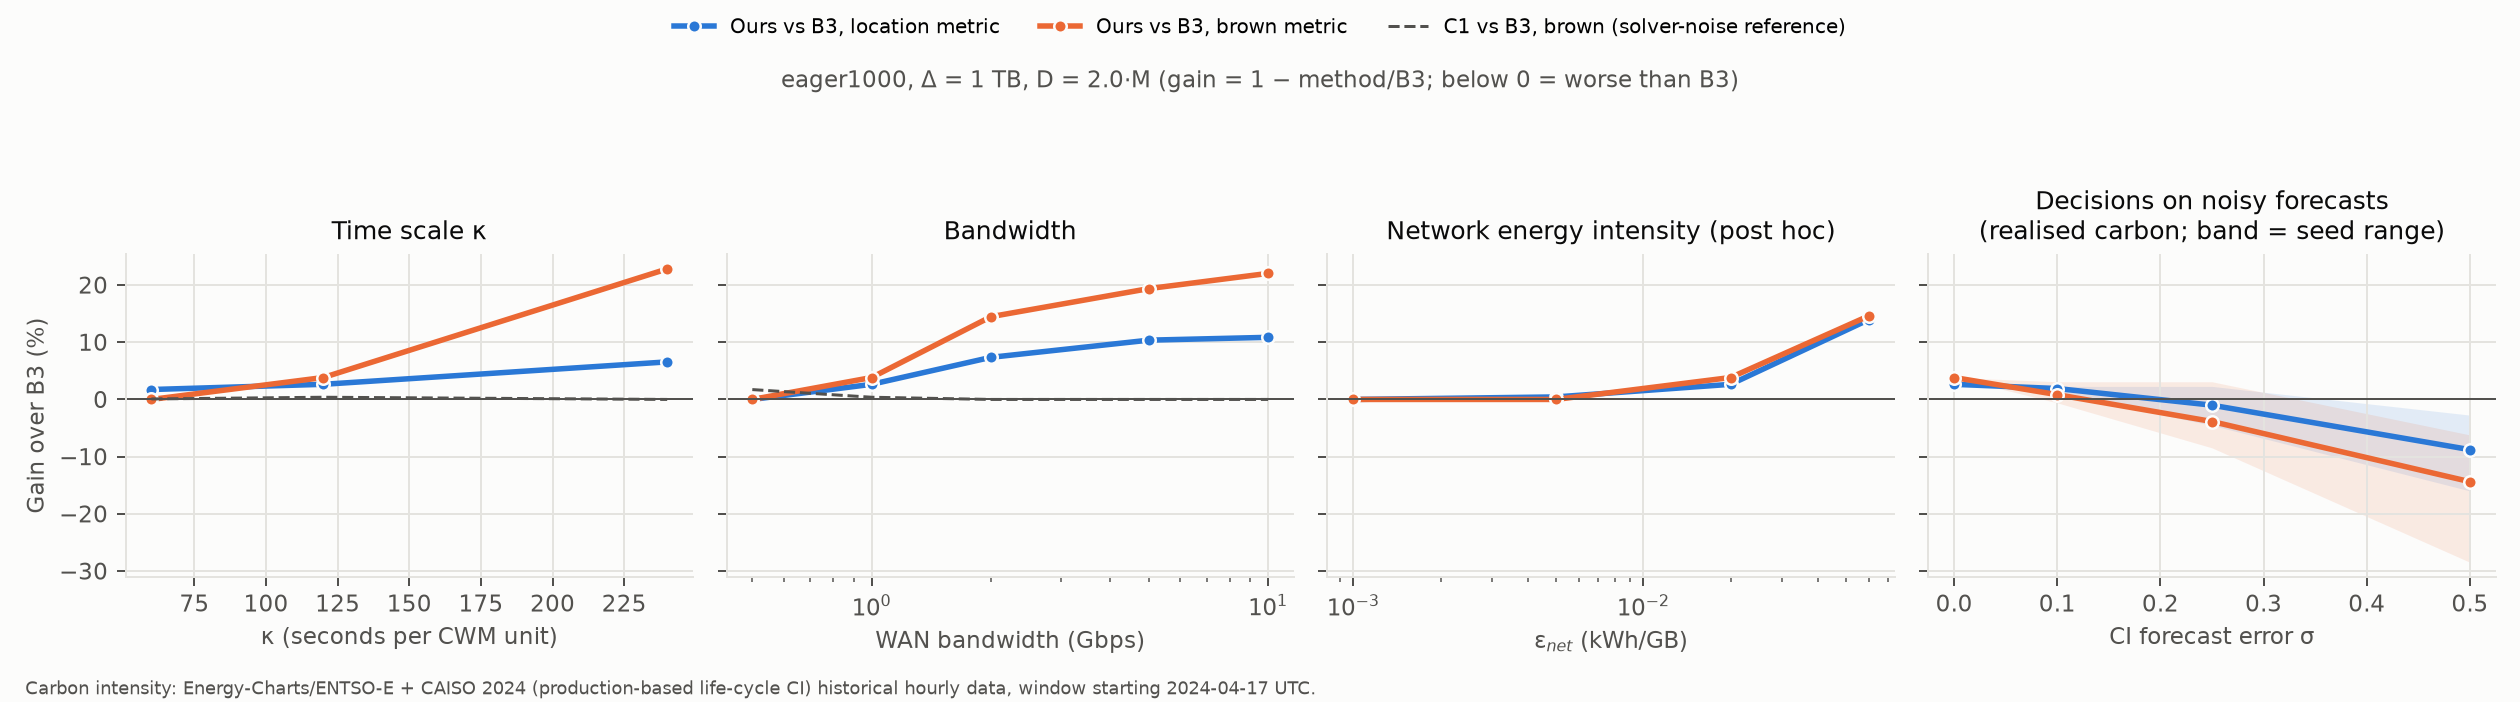
\includegraphics[width=\textwidth,keepaspectratio]{media/media/image7.png}
\caption[Sensitivity to time unit, bandwidth, network energy and forecast error]{Sensitivity to time unit, bandwidth, network energy and forecast error. Gain of Ours over Greenest-DC (B3) as the time unit \ensuremath{\kappa}, bandwidth, network energy \ensuremath{\varepsilon} and forecast error vary (eager1000, 1 TB, \ensuremath{\alpha} = 2). The dashed line is the solver-noise reference (C1); below zero Ours is worse than Greenest-DC.}\label{fig:6.4}
\end{figure}

\section{Why is the gain small?}\label{sec:6.2}

\textbf{Because the cleanest grids are also the flattest, so once a job
moves there, there is little left to gain by waiting.}

Fig.~\ref{fig:6.5} shows the reason. Oslo (hydro) and Paris (nuclear) have
median daily carbon-intensity changes of only 3 and 10 gCO\textsubscript{2}/kWh. The
other three regions vary by 158--232 gCO\textsubscript{2}/kWh (Table~\ref{tab:5.1}). On a stable
grid, one hour is almost as clean as the next, so changing the
computation time adds little. The network still reflects some of the
source grid\textquotesingle s variation, which explains where most of
our remaining gains come from. In short, choosing a very clean, stable
location reduces the additional benefit of choosing a particular time.

Fig.~\ref{fig:6.6} confirms the second part of the argument, Proposition 3. The
most that delaying a transfer can save falls from about 61~\% of its
average for short transfers to 46~\% for a 10-hour transfer and 26~\%
for a 24-hour one. A pure daily cycle predicts the fall but not the
remaining floor, which comes from weather that does not repeat daily.

\begin{figure}[htbp]
\centering
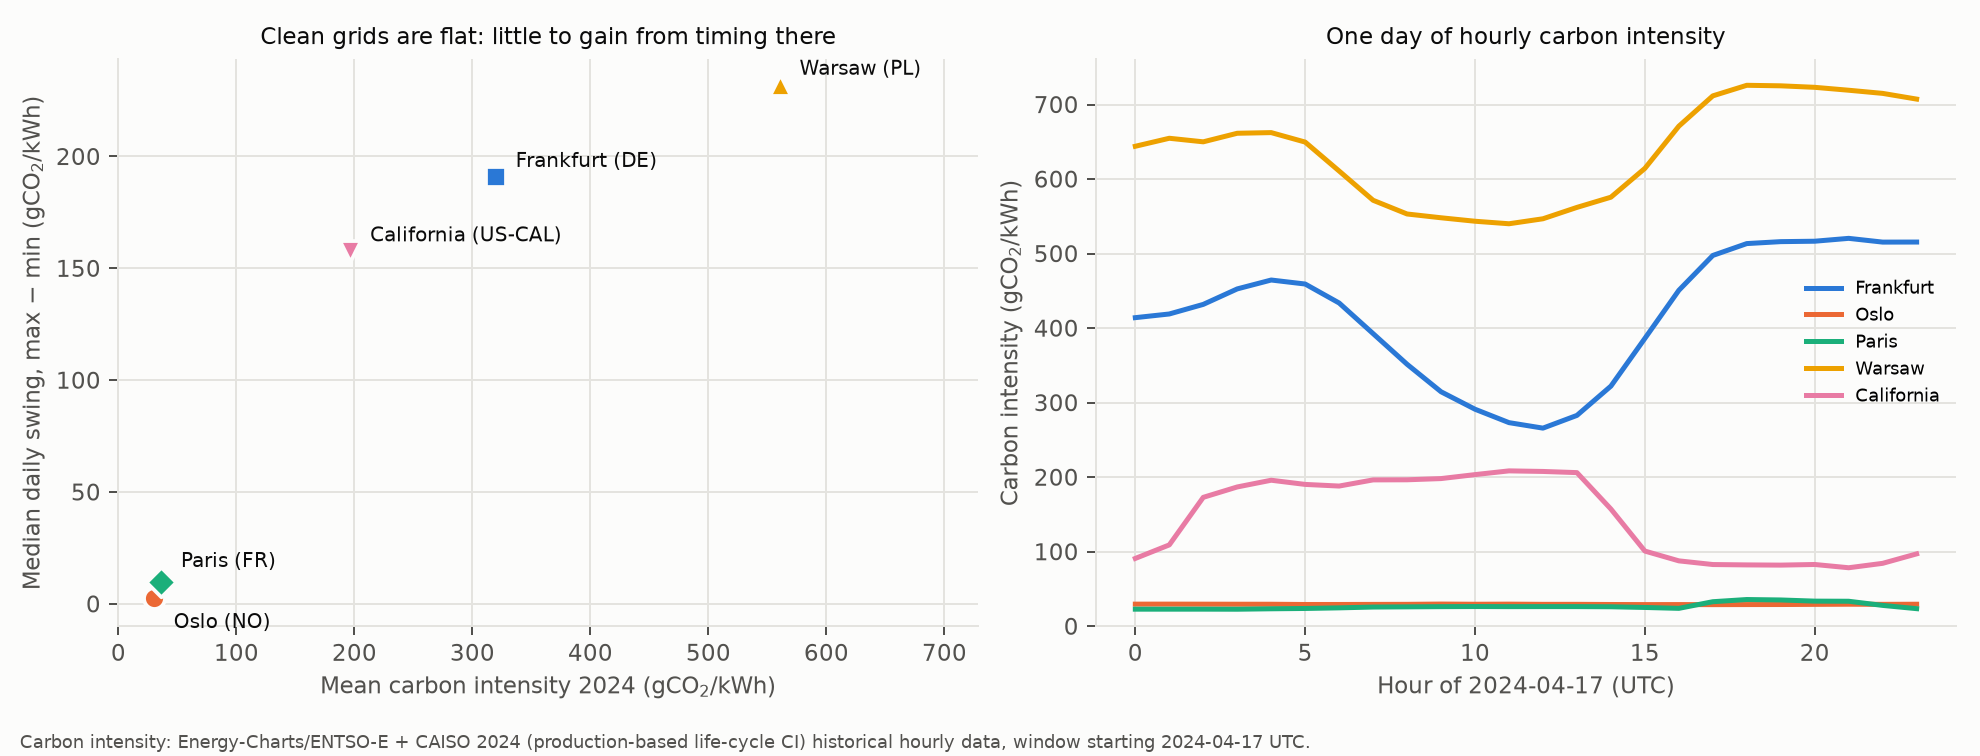
\includegraphics[width=\textwidth,keepaspectratio]{media/media/image8.png}
\caption[Clean grids are flat: carbon intensity versus daily swing]{Clean grids are flat: carbon intensity versus daily swing. The mechanism. Left: mean carbon intensity against median daily swing in 2024; the cleanest grids are the flattest. Right: one day of hourly carbon intensity in the five regions.}\label{fig:6.5}
\end{figure}

\begin{figure}[htbp]
\centering
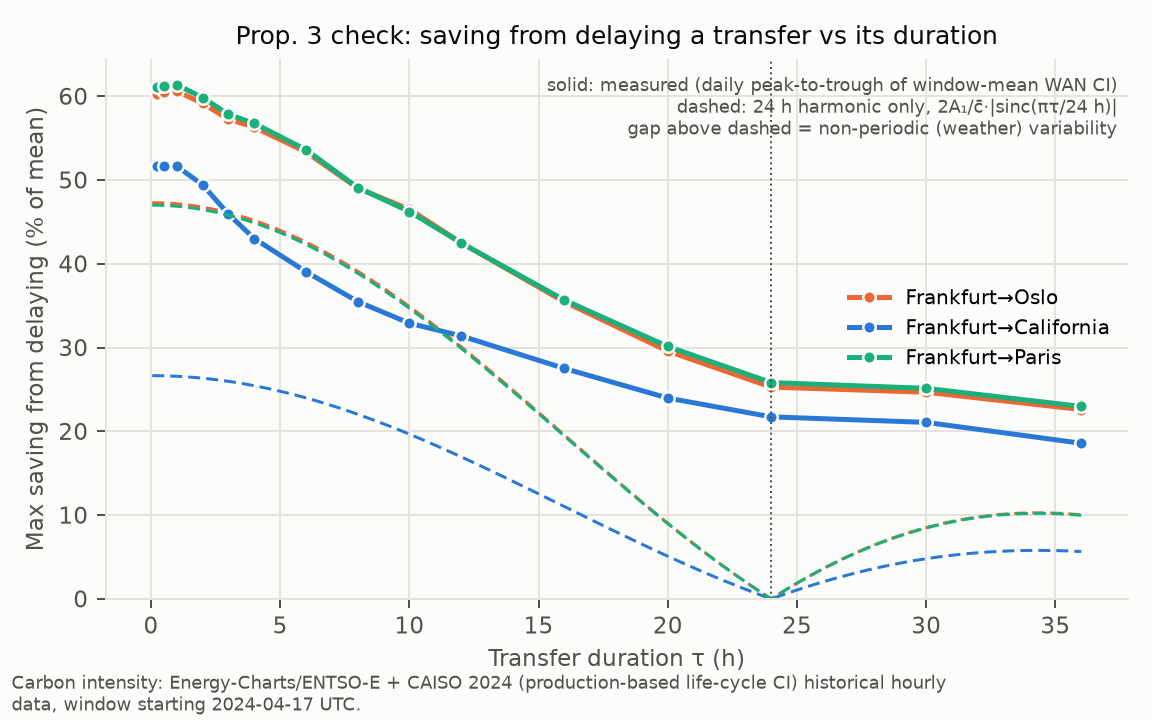
\includegraphics[width=5.6in,keepaspectratio]{media/media/image9.png}
\caption[Longer transfers gain less from waiting]{Longer transfers gain less from waiting. Proposition 3 on real data: the most that delaying a transfer can save, against the transfer\textquotesingle s duration (solid), and the prediction of a pure 24-hour cycle (dashed).}\label{fig:6.6}
\end{figure}

\section{When does it pay off?}\label{sec:6.3}

\textbf{When no flat clean grid is available, the gain triples.}

To test this explanation, we repeated the same 192 problems but allowed
only Frankfurt, Warsaw and California. These three regions have larger
daily changes in carbon intensity. This also represents practical cases
where data-protection rules, contracts or capacity limits prevent a
workflow from using the cleanest locations. We expected joint
optimisation to provide a larger improvement in this setting.

The results support this expectation (Table~\ref{tab:6.3}). The average
improvement over Greenest-DC rises from 1.8\% to 5.3\%, nearly three
times as much. The average saving per job rises from 0.07 kg to 0.95 kg,
about 13 times as much. In 96 of the 139 problems where the two settings
differed, the improvement was larger without the stable clean grids
(paired sign test, p = 8\ensuremath{{}\times 10^{-6}}). The result also holds when network
energy is assumed to be very low: the improvement rises from 1.1\% to
5.0\% at \ensuremath{\varepsilon} = 0.001 (p = 1\ensuremath{{}\times 10^{-8}}). These results support the explanation
that transfer timing matters more when no consistently clean grid is
available.

\begin{table}[htbp]
\centering
\caption[Without a flat clean grid]{Without a flat clean grid. The same 192 problems with all five DCs, and with only Frankfurt, Warsaw and California.}\label{tab:6.3}
\begin{tabular}{@{}
  >{\raggedright\arraybackslash}p{(\columnwidth - 12\tabcolsep) * \real{0.1142}}
  >{\raggedright\arraybackslash}p{(\columnwidth - 12\tabcolsep) * \real{0.1667}}
  >{\raggedright\arraybackslash}p{(\columnwidth - 12\tabcolsep) * \real{0.1257}}
  >{\raggedright\arraybackslash}p{(\columnwidth - 12\tabcolsep) * \real{0.1144}}
  >{\raggedright\arraybackslash}p{(\columnwidth - 12\tabcolsep) * \real{0.1361}}
  >{\raggedright\arraybackslash}p{(\columnwidth - 12\tabcolsep) * \real{0.1563}}
  >{\raggedright\arraybackslash}p{(\columnwidth - 12\tabcolsep) * \real{0.1866}}@{}}
\toprule\noalign{}
\begin{minipage}[b]{\linewidth}\raggedright
\textbf{\ensuremath{\varepsilon} (kWh/GB)}
\end{minipage} & \begin{minipage}[b]{\linewidth}\raggedright
\textbf{Candidate DCs}
\end{minipage} & \begin{minipage}[b]{\linewidth}\raggedright
\textbf{Gain vs Greenest-DC~\%}
\end{minipage} & \begin{minipage}[b]{\linewidth}\raggedright
\textbf{Share \ensuremath{\geq}~5~\%}
\end{minipage} & \begin{minipage}[b]{\linewidth}\raggedright
\textbf{Value of waiting~\%}
\end{minipage} & \begin{minipage}[b]{\linewidth}\raggedright
\textbf{Saving vs Greenest-DC (kg/job)}
\end{minipage} & \begin{minipage}[b]{\linewidth}\raggedright
\textbf{Paired sign test}
\end{minipage} \\
\midrule\noalign{}
0.02 & all five & 1.8 & 11~\% & 1.6 & 0.07 & \\
0.02 & DE, PL, US-CAL & \textbf{5.3} & \textbf{24~\%} & \textbf{3.6} &
\textbf{0.95} & 96/139, p = 8\ensuremath{{}\times 10^{-6}} \\
0.001 & all five & 1.1 & 9~\% & 0.8 & 0.02 & \\
0.001 & DE, PL, US-CAL & \textbf{5.0} & \textbf{21~\%} & \textbf{4.4} &
\textbf{0.77} & 96/128, p = 1\ensuremath{{}\times 10^{-8}} \\
\bottomrule
\end{tabular}
\end{table}

\section{Does it hold under harder conditions?}\label{sec:6.4}

The method also performs consistently in the three harder settings we
tested: different hardware, data-centre queues, and different data
origins (Table~\ref{tab:6.4}). In each setting, we compare it with Greenest-DC and
with a baseline that accounts for the relevant condition, such as
hardware efficiency or queue length.

\begin{table}[htbp]
\centering
\caption[Stress tests: hardware, queues and data origin]{Stress tests: gain of Ours over Greenest-DC and over the fair rival for each setting.}\label{tab:6.4}
\begin{tabular}{@{}
  >{\raggedright\arraybackslash}p{(\columnwidth - 8\tabcolsep) * \real{0.1999}}
  >{\raggedright\arraybackslash}p{(\columnwidth - 8\tabcolsep) * \real{0.3000}}
  >{\raggedright\arraybackslash}p{(\columnwidth - 8\tabcolsep) * \real{0.1199}}
  >{\raggedright\arraybackslash}p{(\columnwidth - 8\tabcolsep) * \real{0.1199}}
  >{\raggedright\arraybackslash}p{(\columnwidth - 8\tabcolsep) * \real{0.2602}}@{}}
\toprule\noalign{}
\begin{minipage}[b]{\linewidth}\raggedright
\textbf{Study (fair rival)}
\end{minipage} & \begin{minipage}[b]{\linewidth}\raggedright
\textbf{Setting}
\end{minipage} & \begin{minipage}[b]{\linewidth}\raggedright
\textbf{vs Greenest-DC~\%}
\end{minipage} & \begin{minipage}[b]{\linewidth}\raggedright
\textbf{vs fair rival~\%}
\end{minipage} & \begin{minipage}[b]{\linewidth}\raggedright
\textbf{Note}
\end{minipage} \\
\midrule\noalign{}
Hardware (Efficiency-aware) & All DCs standard & 2.0 & 2.0 & \\
& Oslo and Paris efficient & 2.8 & 2.8 & \\
& Oslo and Paris legacy; Warsaw and California efficient & 1.9 & 1.9 &
Clean grids still win \\
& Oslo legacy; California efficient & \textbf{9.1} & 1.4 & Greenest-DC
picks the wrong clean grid \\
Queues (Queue-aware) & No queues & 1.7 & 1.7 & \\
& Moderate (\ensuremath{\rho} = 1) & 1.2 & 1.2 & \\
& Heavy (\ensuremath{\rho} = 2) & 1.0 & 2.1 & Greenest-DC misses the deadline in 6~\% \\
Data origin (No-wait) & Data starts in Frankfurt & 1.7 & 1.6 & Saved by
waiting: 0.076 kg/job \\
& Data starts in Warsaw & 2.2 & 2.1 & 0.144 kg/job \\
& Data starts in California & 3.0 & 2.9 & 0.134 kg/job \\
\bottomrule
\end{tabular}
\end{table}

\subsection{Different hardware}

Real data centres differ in processor efficiency and cooling, so the
location with the cleanest electricity is not always the location with
the lowest total emissions. We tested cases where hardware efficiency
and grid cleanliness disagree. When Oslo used legacy hardware,
Greenest-DC still selected it and produced 9.1\% more emissions on
average than Ours. The Efficiency-aware baseline, which accounts for
power usage effectiveness (PUE), avoided most of this difference; Ours
improved on it by 1.4\%. In the other tested hardware combinations, the
clean grids remained preferable because their carbon intensity was much
lower than that of the other regions. Overall, the benefit of a clean
location remained under the hardware differences we modelled.

\subsection{Busy data centres}

Clean data-centre regions may also be busy, so a queue can reduce the
time left before the deadline. We added daily queues, with the longest
waits during local office hours (09:00--18:00), and varied their
intensity using \ensuremath{\rho}. We expected Ours\textquotesingle{} advantage over
Queue-aware to increase as queues became longer, but it remained between
1.2\% and 2.1\%. Under the heaviest queue setting (\ensuremath{\rho} = 2), Greenest-DC
missed the deadline in 6\% of problems, while Ours did not. Queue-aware
also avoided these misses because it checks queue length before choosing
a data centre. The queues had limited effect on the benefit of waiting
because they were largest at the stable clean grids, where the exact
start time matters less.

\subsection{Where the data starts}

Proposition 3 says waiting should save more when the data starts on a
grid with a big daily swing. We expected the largest saving in kilograms
from Warsaw (largest swing), and the largest relative saving from
California, then Frankfurt, then Warsaw (swing relative to average CI:
0.33, 0.20, 0.15). The first held, narrowly: Warsaw saves 0.144 kg per
job against California\textquotesingle s 0.134. The second held only
partly: California is highest as predicted, but Warsaw comes out ahead
of Frankfurt. The theory gets the main effect right but not the finer
ordering, which also depends on how regular each grid\textquotesingle s
daily cycle is.

\subsection{The cost of waiting and of a longer deadline}

Almost all of Ours\textquotesingle{} advantage comes from waiting, and
our model treats waiting as free. In reality the input sits on disks
while the job waits, so we charged every strategy a constant
\emph{holding power} from submission until computing starts, and
recomputed every choice from the saved results (with zero holding power,
the original results come back exactly). Fig.~\ref{fig:6.7} shows that this
changes almost nothing. Keeping 0.1--1 TB on disk takes roughly 0.1--20
W. At 10 W the value of waiting falls only from 1.57~\% to 1.43~\% over
the year, and from 3.55~\% to 3.53~\% without a flat clean grid. Waiting
stops paying only at about 0.9 kW (year-round) to 8.6 kW (no flat grid),
that is, if whole servers were kept reserved, which no strategy here
does. And because Greenest-DC, No-wait and Queue-aware are among
Ours\textquotesingle{} own candidates, Ours can never fall below them:
with high holding power it simply stops waiting.

\begin{figure}[htbp]
\centering
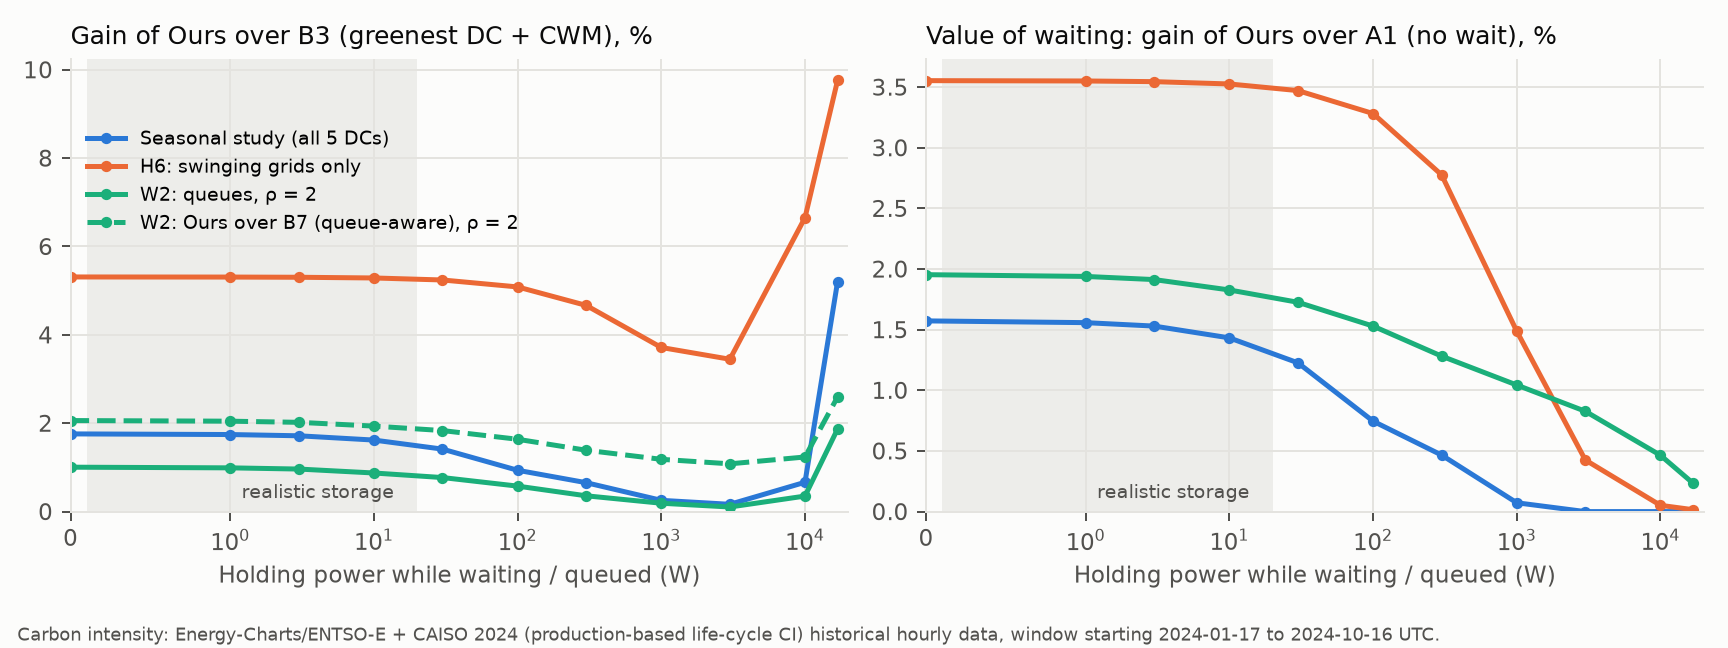
\includegraphics[width=\textwidth,keepaspectratio]{media/media/image10.png}
\caption[Effect of charging for the time spent waiting]{Effect of charging for the time spent waiting. Holding emissions: gain of Ours over Greenest-DC (B3, left) and value of waiting, i.e. gain over No-wait (A1, right), when every strategy pays a holding power P from submission until computing starts. The shaded band is realistic storage power for these inputs.}\label{fig:6.7}
\end{figure}

A longer deadline is the other cost of waiting. CWM stretches each
schedule to fill its window (median 99.8~\% of it), so every job
finishes right at its deadline, and the real trade-off is carbon against
deadline. Between deadline factors of 1.5 and 2.5, staying in Frankfurt
saves up to 1.5 kg CO\textsubscript{2} per extra hour of deadline, but at a clean DC an
extra hour is worth at most 0.17 kg. Moving to a clean grid makes
deadline slack, like timing, much less valuable. For the short
atacseq200 workflow only Ours turns extra slack into savings (36 g per
hour at 1 TB; Greenest-DC sends at once and gains nothing).

The workflows also differ. CWM beats HEFT by about 19--20~\% on the
three 1000-task workflows but by only 0.7~\% on atacseq200. The joint
gain over Greenest-DC is larger for atacseq200 (2.8--3.1~\%) than for
eager1000 (0.3--0.9~\%). Waiting saves about the same grams of network
carbon for both, but eager1000 uses much more compute energy, which
dilutes the saving, and its longer schedule loses some compute carbon
when it waits.

\section{Can a cheap rule get most of it?}\label{sec:6.5}

\textbf{Yes: checking 3--4 candidates instead of about 64 recovers most
of the gain.}

Table~\ref{tab:6.5} measures the \emph{capture} of the cheap rule: the share of
Ours\textquotesingle{} gain over the best simple strategy that the rule
also achieves. Over the year, the top-3 rule captures 76~\% with at most
4 solver calls instead of 64 on average (6~\% of the work). It picks
exactly Ours\textquotesingle{} choice in 70~\% of problems and is never
more than 5.5~\% behind. We had aimed for 80~\%, so it falls just short
there. On the studies it had never seen, capture ranges from 54~\% to
85~\%, and it is highest, 85~\%, exactly where joint scheduling matters
most: without a flat clean grid.

\begin{table}[htbp]
\centering
\caption[Cheap rule: captured gain and solver calls]{Cheap rule: share of Ours\textquotesingle{} gain over the best simple strategy that it captures, and solver calls.}\label{tab:6.5}
\begin{tabular}{@{}
  >{\raggedright\arraybackslash}p{(\columnwidth - 10\tabcolsep) * \real{0.2526}}
  >{\raggedright\arraybackslash}p{(\columnwidth - 10\tabcolsep) * \real{0.1684}}
  >{\raggedright\arraybackslash}p{(\columnwidth - 10\tabcolsep) * \real{0.1368}}
  >{\raggedright\arraybackslash}p{(\columnwidth - 10\tabcolsep) * \real{0.1368}}
  >{\raggedright\arraybackslash}p{(\columnwidth - 10\tabcolsep) * \real{0.1368}}
  >{\raggedright\arraybackslash}p{(\columnwidth - 10\tabcolsep) * \real{0.1687}}@{}}
\toprule\noalign{}
\begin{minipage}[b]{\linewidth}\raggedright
\textbf{Study}
\end{minipage} & \begin{minipage}[b]{\linewidth}\raggedright
\textbf{Compared with}
\end{minipage} & \begin{minipage}[b]{\linewidth}\raggedright
\textbf{Top-1 capture}
\end{minipage} & \begin{minipage}[b]{\linewidth}\raggedright
\textbf{Top-3 capture}
\end{minipage} & \begin{minipage}[b]{\linewidth}\raggedright
\textbf{Top-3 = Ours}
\end{minipage} & \begin{minipage}[b]{\linewidth}\raggedright
\textbf{Solver calls, top-3 / Ours}
\end{minipage} \\
\midrule\noalign{}
Year-round (tuned on) & Greenest-DC & 70~\% & \textbf{76~\%} & 70~\% &
\ensuremath{\leq}~4 / 64 \\
No flat clean grid & Greenest-DC & -- & \textbf{85~\%} & -- & \ensuremath{\leq}~4 /
33 \\
Hardware & Efficiency-aware & 39~\% & 55~\% & 76~\% & \ensuremath{\leq}~4 / 65 \\
Queues, \ensuremath{\rho} = 0 / 1 / 2 & Queue-aware & 64 / 54 / 80~\% & 68 / 54 / 84~\%
& 64 / 78 / 70~\% & \ensuremath{\leq}~4 / 81 \\
\bottomrule
\end{tabular}
\end{table}

\section{What happened to our expectations}\label{sec:6.6}

Table~\ref{tab:6.6} lists each expectation we wrote down before running, and the
outcome. Two held, two held partly, one was narrowly missed and one did
not hold.

\begin{table}[htbp]
\centering
\caption[Expectations and outcomes]{Expectations written down before running, and their outcomes.}\label{tab:6.6}
\begin{tabular}{@{}
  >{\raggedright\arraybackslash}p{(\columnwidth - 2\tabcolsep) * \real{0.5000}}
  >{\raggedright\arraybackslash}p{(\columnwidth - 2\tabcolsep) * \real{0.5000}}@{}}
\toprule\noalign{}
\begin{minipage}[b]{\linewidth}\raggedright
\textbf{Expectation}
\end{minipage} & \begin{minipage}[b]{\linewidth}\raggedright
\textbf{Outcome}
\end{minipage} \\
\midrule\noalign{}
Hardware: Greenest-DC loses \ensuremath{\geq}~10~\% when hardware and CI disagree &
Partly: only between the two clean grids (9.1~\% in the ``mixed'' case);
Efficiency-aware recovers it \\
Queues: the gain over Queue-aware grows with busyness & Did not hold
(1.2--2.1~\%) \\
Data origin: largest saving in kg when data starts in Warsaw & Held,
narrowly \\
Data origin: relative saving California \textgreater{} Frankfurt
\textgreater{} Warsaw & Partly: California highest, but Warsaw
\textgreater{} Frankfurt \\
Cheap rule: \ensuremath{\geq}~80~\% capture with \ensuremath{\leq}~10~\% of the solver calls & Narrowly
missed over the year (76~\% at 6~\%); met without a flat grid (85~\%) \\
No flat clean grid: the gain is larger & \textbf{Held} (1.8~\% \ensuremath{\rightarrow} 5.3~\%,
p = 8\ensuremath{{}\times 10^{-6}}) \\
\bottomrule
\end{tabular}
\end{table}

\section{Discussion}\label{sec:6.7}

The results show that location choice provides most of the carbon
savings. Ours emits 83.9\% less than staying at the source and 16.1\%
less than using the greenest data centre with a carbon-unaware schedule.
The additional benefit of timing depends on how stable the available
grids are: it is 1.8\% across the year when Oslo and Paris are
available, and 5.3\% when they are excluded. In the tested scenarios,
Ours meets the deadline and is never worse than the baseline strategies
included in its candidate set. In the harder hardware and queue
settings, its improvement over the corresponding informed baselines is
smaller, between 1.2\% and 2.8\%.

A useful way to understand the result is to think of a stable clean grid
as a resource that is already low-carbon at almost every hour. Once a
workflow is sent there, waiting for a cleaner hour has little value.
Joint scheduling is more useful when all available grids change
substantially during the day, because it can then choose both a better
location and a better transfer time. In practice, a simple
greenest-data-centre strategy may be sufficient when a stable clean grid
is available; otherwise, the joint search or its cheaper ranking rule
can provide additional savings.

\section{Comparison with existing research}\label{sec:6.8}

Table~\ref{tab:6.7} puts our findings next to results reported in earlier work.
The settings, data and measures differ, so we compare the direction of
each effect rather than the exact numbers.

\begin{table}[htbp]
\centering
\caption[Comparison with results reported in earlier work]{Comparison with results reported in earlier work. Our findings beside results reported in earlier work (direction of each effect).}\label{tab:6.7}
\begin{tabular}{@{}
  >{\raggedright\arraybackslash}p{(\columnwidth - 4\tabcolsep) * \real{0.2221}}
  >{\raggedright\arraybackslash}p{(\columnwidth - 4\tabcolsep) * \real{0.3555}}
  >{\raggedright\arraybackslash}p{(\columnwidth - 4\tabcolsep) * \real{0.4224}}@{}}
\toprule\noalign{}
\begin{minipage}[b]{\linewidth}\raggedright
\textbf{Claim}
\end{minipage} & \begin{minipage}[b]{\linewidth}\raggedright
\textbf{Reported in earlier work}
\end{minipage} & \begin{minipage}[b]{\linewidth}\raggedright
\textbf{This work}
\end{minipage} \\
\midrule\noalign{}
Carbon-aware scheduling beats carbon-agnostic HEFT & CWM: 69~\% lower
carbon cost than carbon-agnostic HEFT-SL, and 42--48~\% lower than
CaWoSched, at the largest deadline flexibility tested (D = 2M) {[}6{]} &
Agrees, but smaller with our carbon measure: CWM beats HEFT by about
19--20~\% on the 1000-task workflows and 0.7~\% on atacseq200; Ours vs
Greenest-DC + HEFT 16.1~\% \\
Region choice dominates spatiotemporal savings & Difference in CI
between regions dominates the savings {[}5{]} & Agrees, and explained:
83.9~\% vs staying local, 1.8~\% from timing; the clean grids are flat
(Section~\ref{sec:6.2}) \\
Waiting pays more on grids that vary more & Savings from waiting depend
on how strongly each grid varies {[}1{]} & Agrees: the value of waiting
follows the source grid\textquotesingle s swing (Section~\ref{sec:6.4}); 5.3~\%
without a flat clean grid (Section~\ref{sec:6.3}) \\
Shifting transfers in time saves carbon & Temporal transfer scheduling
saves carbon while meeting transfer deadlines {[}8{]}, {[}9{]} & Agrees
for the network (\ensuremath{-}12.4 kg network vs +0.6 kg compute on the winners),
but optimising the transfer alone (Network-only) loses 4.9~\% to Ours \\
Network energy per GB & \ensuremath{\approx}~0.06 kWh/GB in 2015, halving about every two
years {[}7{]} & We vary it from 0.001 to 0.06; the no-flat-grid result
holds at 0.001 (1.1~\% \ensuremath{\rightarrow} 5.0~\%) \\
\bottomrule
\end{tabular}
\end{table}

\chapter{Discussion and Limitations}\label{ch:7}

\section{Implications}\label{sec:7.1}

For a deadline-constrained workflow, if a clean and stable grid is
available, a practical strategy is to transfer the data there promptly
and let a carbon-aware scheduler place the tasks. In our experiments,
joint optimisation added about 2\% on average over sending the data
immediately to the cleanest data centre. If the available grids all vary
substantially during the day---for example, because of data-protection
rules, contracts or capacity limits---joint scheduling becomes more
valuable. In that setting, its improvement was about three times larger,
and the cheap ranking rule captured most of that benefit with only a few
solver calls.

The benefit of flexible timing therefore depends strongly on the
electricity grid at the destination. Location and transfer time should
be considered together rather than optimised independently.

\section{Limitations}\label{sec:7.2}

\begin{itemize}
\item
  \textbf{Network energy.} We charge the network a fixed energy per GB.
  Network carbon is a large part of many totals (at 1 TB,
  Greenest-DC\textquotesingle s network carbon is about 4.3 kg), so this
  assumption matters. We report the whole range and show the key result
  holds even at \ensuremath{\varepsilon} = 0.001.
\item
  \textbf{Carbon data.} Our CI counts what each country generates, not
  what it imports, so Poland and Germany are probably somewhat
  underestimated. The network\textquotesingle s CI is the average of its
  two ends and ignores the countries in between.
\item
  \textbf{Illustrative scenarios.} The hardware types and queue patterns
  are reasonable scenarios fixed before running, not measurements from
  real data centres.
\item
  \textbf{Coverage.} The year-round study covers four days, one per
  season, and most studies use one solver seed. The noise control covers
  the year-round winners, and an earlier 12-day run behaved the same way
  in each season.
\item
  \textbf{Simplifications.} Constant dedicated bandwidth, no results
  sent back, one workflow at a time, and perfect knowledge of future CI
  except in the forecast test, where noisy forecasts were the
  method\textquotesingle s clearest weakness.
\end{itemize}

\chapter{Summary and Conclusions}\label{ch:8}

This project extended CWM, a carbon-aware workflow scheduler for a
single data centre, to multiple data centres. The extended system
jointly chooses where a workflow should run, when its input should be
transferred, and how its tasks should be scheduled, while meeting one
shared deadline.

The problem has useful structure. Waiting cannot improve the best
possible compute-carbon result because it leaves less time before the
deadline. With hourly carbon-intensity data, only a small set of
transfer start times needs to be checked. Also, longer transfers
generally gain less from waiting. We used these properties to build a
search around the CWM solver.

Experiments using real 2024 electricity data show that choosing a clean
data-centre location provides most of the benefit. The additional gain
from choosing the transfer time is modest (1.8\%) when stable clean
grids are available, because their carbon intensity changes very little
during the day. When these grids are unavailable, the gain rises to
5.3\%. The main explanation also held in our tests with different
hardware, queues and network-energy assumptions. A simpler ranking rule
captured 76--85\% of the full optimiser\textquotesingle s improvement
using at most four solver calls.

Overall, this work contributes a joint formulation and analysis of the
scheduling problem, an implementation built around CWM, an evaluation using real electricity data and several stress
tests, and a lower-cost rule that retains most of the benefit of the
full search. The results show why choosing both the data-centre location
and transfer time can reduce the carbon emissions of
deadline-constrained scientific workflows.

\chapter{Scope for Future Work}\label{ch:9}

Several directions remain open:

\begin{itemize}
\item
  \textbf{Decisions that tolerate bad forecasts:} wait only when the
  forecast saving clearly exceeds the forecast\textquotesingle s
  uncertainty, to avoid the losses we saw with noisy forecasts.
\item
  \textbf{A carbon-based objective inside CWM}, so that the inner
  scheduler optimises the same measure we report.
\item
  \textbf{Better data:} carbon intensity that includes imports, more
  regions (including India), and measured queue and hardware data from
  real data centres.
\item
  \textbf{Many workflows at once}, sharing DCs and links. If every job
  goes to the greenest DC, its queue grows with that choice; our fixed
  queues (Section~\ref{sec:6.4}) do not capture this, and it would hurt
  greenest-first placement the most.
\item
  \textbf{Splitting a workflow across DCs}, and streaming the input so
  that computing can start before the transfer has finished.
\end{itemize}

\chapter*{References}\addcontentsline{toc}{chapter}{References}
\sloppy
\begin{enumerate}[label={[\arabic*]}, leftmargin=2.6em, labelsep=0.6em, itemsep=4pt]
\item P. Wiesner, I. Behnke, D. Scheinert, K. Gontarska, and L. Thamsen, ``Let\textquotesingle s wait awhile: How temporal workload shifting can reduce carbon emissions in the cloud,'' in \emph{Proc. 22nd Int. Middleware Conf.}, 2021, doi: 10.1145/3464298.3493399.
\item W. A. Hanafy, Q. Liang, N. Bashir, D. Irwin, and P. Shenoy, ``CarbonScaler: Leveraging cloud workload elasticity for optimizing carbon-efficiency,'' \emph{Proc. ACM Meas. Anal. Comput. Syst.}, vol. 7, no. 3, art. 57, Dec. 2023, doi: 10.1145/3626788.
\item A. Radovanović \emph{et al.}, ``Carbon-aware computing for datacenters,'' \emph{arXiv preprint} arXiv:2106.11750, 2021.
\item A. Souza, S. Jasoria, B. Chakrabarty, A. Bridgwater, A. Lundberg, F. Skogh, A. Ali-Eldin, D. Irwin, and P. Shenoy, ``CASPER: Carbon-aware scheduling and provisioning for distributed web services,'' in \emph{Proc. 14th Int. Green and Sustainable Computing Conf. (IGSC)}, 2023, pp. 67--73, doi: 10.1145/3634769.3634812.
\item M. Zanotto, L. Vicentini, R. Vreto, F. Lumpp, D. Braga, and S. Fiore, ``A user-centric Kubernetes-based architecture for green cloud computing,'' \emph{arXiv preprint} arXiv:2509.13325, 2025.
\item D. Schweisgut, A. Benoit, Y. Robert, and H. Meyerhenke, ``Carbon-aware mapping and scheduling for deadline-constrained workflows,'' \emph{arXiv preprint} arXiv:2605.27652, 2026.
\item J. Aslan, K. Mayers, J. G. Koomey, and C. France, ``Electricity intensity of internet data transmission: Untangling the estimates,'' \emph{J. Ind. Ecol.}, vol. 22, no. 4, pp. 785--798, 2018.
\item E. Rodrigues, J. Goldverg, and T. Kosar, ``Carbon-aware temporal data transfer scheduling across cloud datacenters,'' \emph{arXiv preprint} arXiv:2506.04117, 2025.
\item J. Goldverg, H. Jamil, E. Rodriguez, and T. Kosar, ``Carbon-aware end-to-end data movement,'' \emph{arXiv preprint} arXiv:2406.09650, 2024.
\item H. Topcuoglu, S. Hariri, and M.-Y. Wu, ``Performance-effective and low-complexity task scheduling for heterogeneous computing,'' \emph{IEEE Trans. Parallel Distrib. Syst.}, vol. 13, no. 3, pp. 260--274, 2002.
\item D. Schweisgut, A. Benoit, Y. Robert, and H. Meyerhenke, ``Carbon-aware workflow scheduling with fixed mapping and deadline constraint,'' in \emph{Proc. 54th Int. Conf. Parallel Processing (ICPP)}, 2025. arXiv:2507.08725.
\item Fraunhofer ISE, ``Energy-Charts: Public net electricity generation,'' 2024 data. {[}Online{]}. Available: \url{https://www.energy-charts.info}. {[}Accessed: 13-Nov-2026{]}.
\item California ISO, ``Today\textquotesingle s Outlook: Supply trend (fuel source history),'' 2024 data. {[}Online{]}. Available: \url{https://www.caiso.com/todays-outlook/supply}. {[}Accessed: 13-Nov-2026{]}.
\item S. Schlömer \emph{et al.}, ``Annex III: Technology-specific cost and performance parameters,'' in \emph{Climate Change 2014: Mitigation of Climate Change. Contribution of Working Group III to the Fifth Assessment Report of the IPCC}. Cambridge, U.K.: Cambridge Univ. Press, 2014.
\item T. Coleman, H. Casanova, L. Pottier, M. Kaushik, E. Deelman, and R. Ferreira da Silva, ``WfCommons: A framework for enabling scientific workflow research and development,'' \emph{Future Gener. Comput. Syst.}, vol. 128, pp. 16--27, 2022.
\item Google, ``2024 Environmental Report,'' 2024. {[}Online{]}. Available: \url{https://sustainability.google/reports/}. {[}Accessed: 13-Nov-2026{]}.
\item Uptime Institute, ``Global Data Center Survey 2024,'' 2024. {[}Online{]}. Available: \url{https://uptimeinstitute.com/resources/research-and-reports}. {[}Accessed: 13-Nov-2026{]}.
\end{enumerate}

\end{document}
